\documentclass[11pt, spanish]{article}
\usepackage[spanish]{babel}
\selectlanguage{spanish}
\usepackage[utf8]{inputenc}
\usepackage{amsmath}
\usepackage{amsfonts}
\usepackage{amsthm}
\usepackage{float}
\usepackage{graphicx}

% Margenes
\usepackage[left=2cm,right=2cm,top=2cm,bottom=2cm]{geometry}
%Espaciado
%\linespread{1.3}


\title{Introducción al Procesamiento Digital de Imágenes - Práctica 2}
\date{}
\author{Gonzalo Ciruelos Rodríguez (LU: 63/14)}

\begin{document}
\maketitle

Para preparar el entorno para poder ejecutar todos los programas,
primero debe tenerse instalado \texttt{python3} (y su \texttt{pip} correspondiente).
Luego, debe ejecutarse 
\begin{verbatim}
    virtualenv -p python3 venv 
    . venv/bin/activate
    pip install -r requirements.txt 
\end{verbatim}

\noindent para instalar las dependencias (pillow (para imágenes), numpy y matplotlib).



\section{Ejercicio 1.}
\subsection{Ejercicio 1.a.}

El histograma de los canales RGB de las imágenes.

Modo de uso
\begin{verbatim}
    python3 ej01-a.py <img>
\end{verbatim}

\subsubsection*{Ejemplos}
\begin{figure}[H]
\centering
  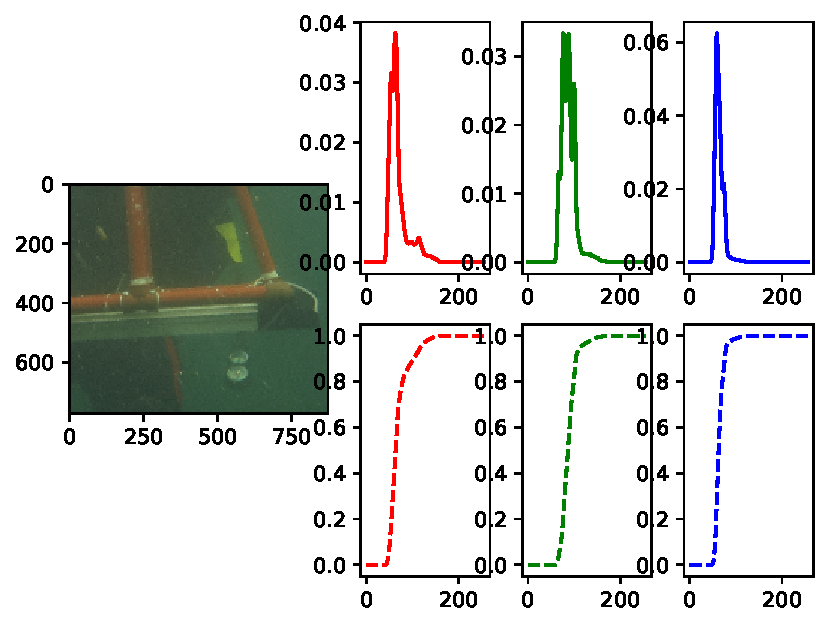
\includegraphics[height=6cm]{informe-imgs/ej01-a-1.pdf}
  \caption{\texttt{python3 practica1/ej01-a.py test/imagenesClaseColor/1907xx.png}}
\end{figure}
\begin{figure}[H]
\centering
  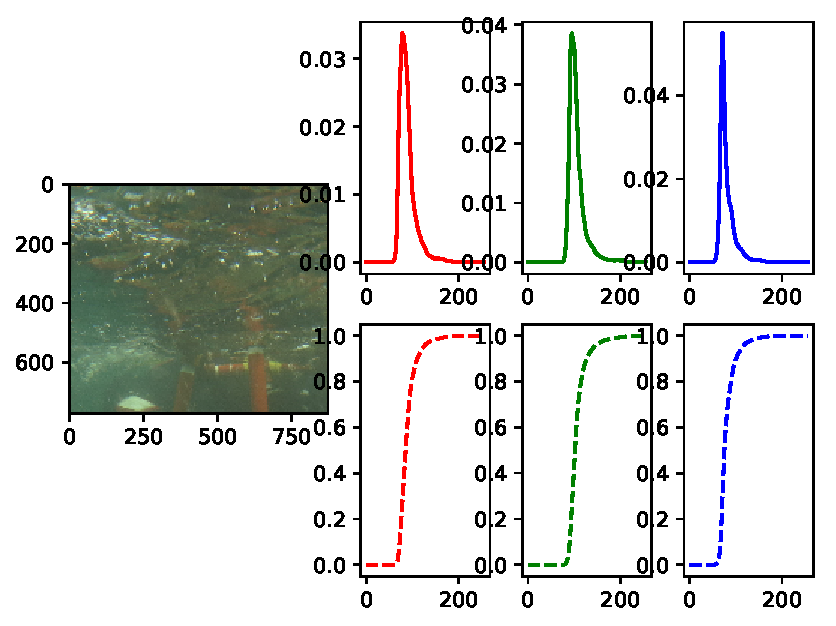
\includegraphics[height=6cm]{informe-imgs/ej01-a-2.pdf}
  \caption{\texttt{python3 practica1/ej01-a.py test/imagenesClaseColor/1908iv.png}}
\end{figure}


\subsection{Ejercicio 1.b.}

Ecualización canal por canal.
Al no aplicarle la misma transoformación a todos los canales (dado que sus histogramas son distintos)
la imágen puede quedar no del todo bien.

Modo de uso
\begin{verbatim}
    python3 ej01-b.py <img>
\end{verbatim}

\subsubsection*{Ejemplos}
\begin{figure}[H]
\centering
  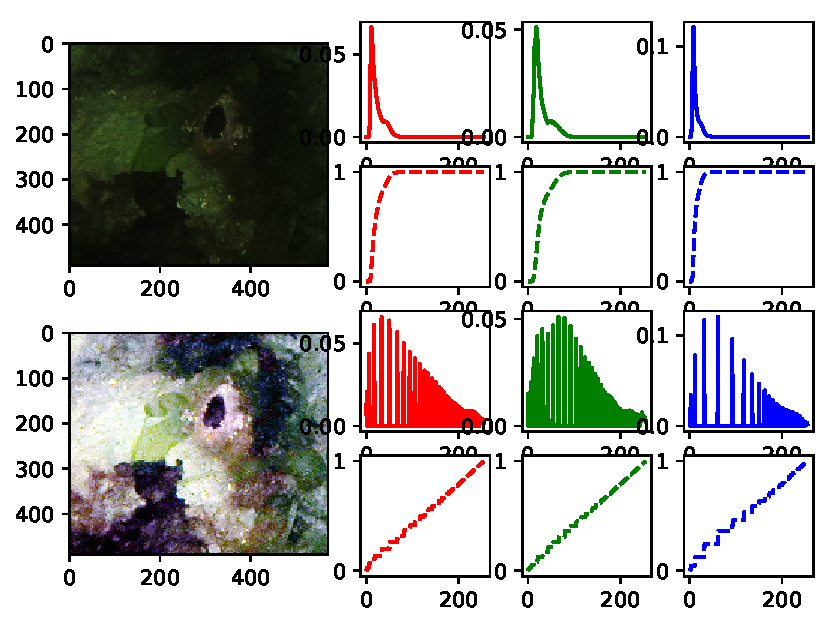
\includegraphics[height=6cm]{informe-imgs/ej01-b-1.pdf}
  \caption{\texttt{python3 practica1/ej01-b.py test/imagenesClaseColor/1906ax.png}}
\end{figure}
\begin{figure}[H]
\centering
  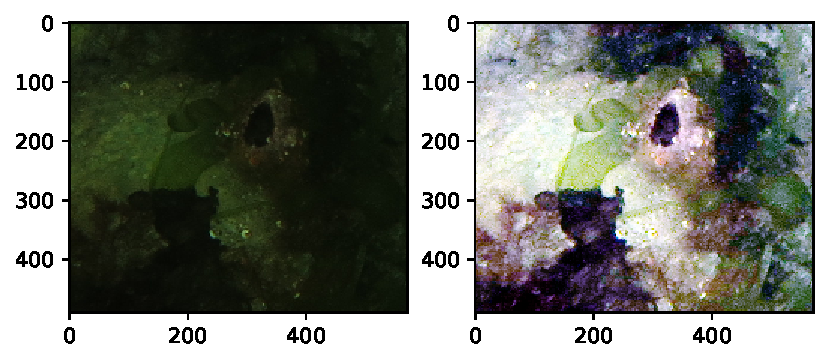
\includegraphics[height=6cm]{informe-imgs/ej01-b-2.pdf}
  \caption{\texttt{python3 practica1/ej01-b.py test/imagenesClaseColor/1906ax.png --end}}
\end{figure}

\begin{figure}[H]
\centering
  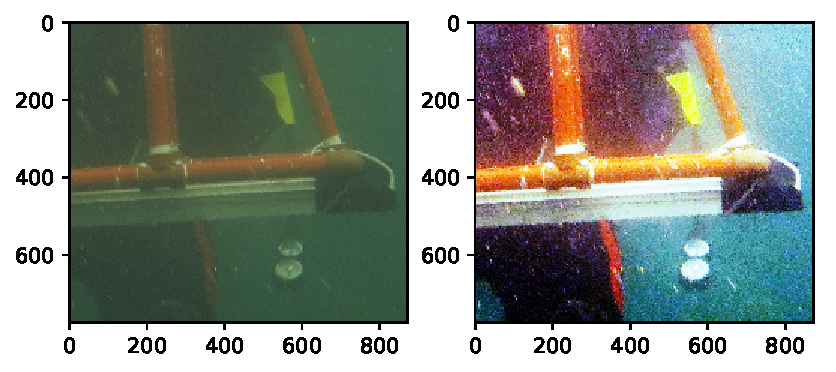
\includegraphics[height=6cm]{informe-imgs/ej01-b-3.pdf}
  \caption{\texttt{python3 practica1/ej01-b.py test/imagenesClaseColor/1907xx.png --end}}
\end{figure}

\subsection{Ejercicio 1.c.}

Pasaje a HSI.

Modo de uso
\begin{verbatim}
    python3 ej01-c.py <img>
\end{verbatim}

\subsubsection*{Ejemplos}
\begin{figure}[H]
\centering
  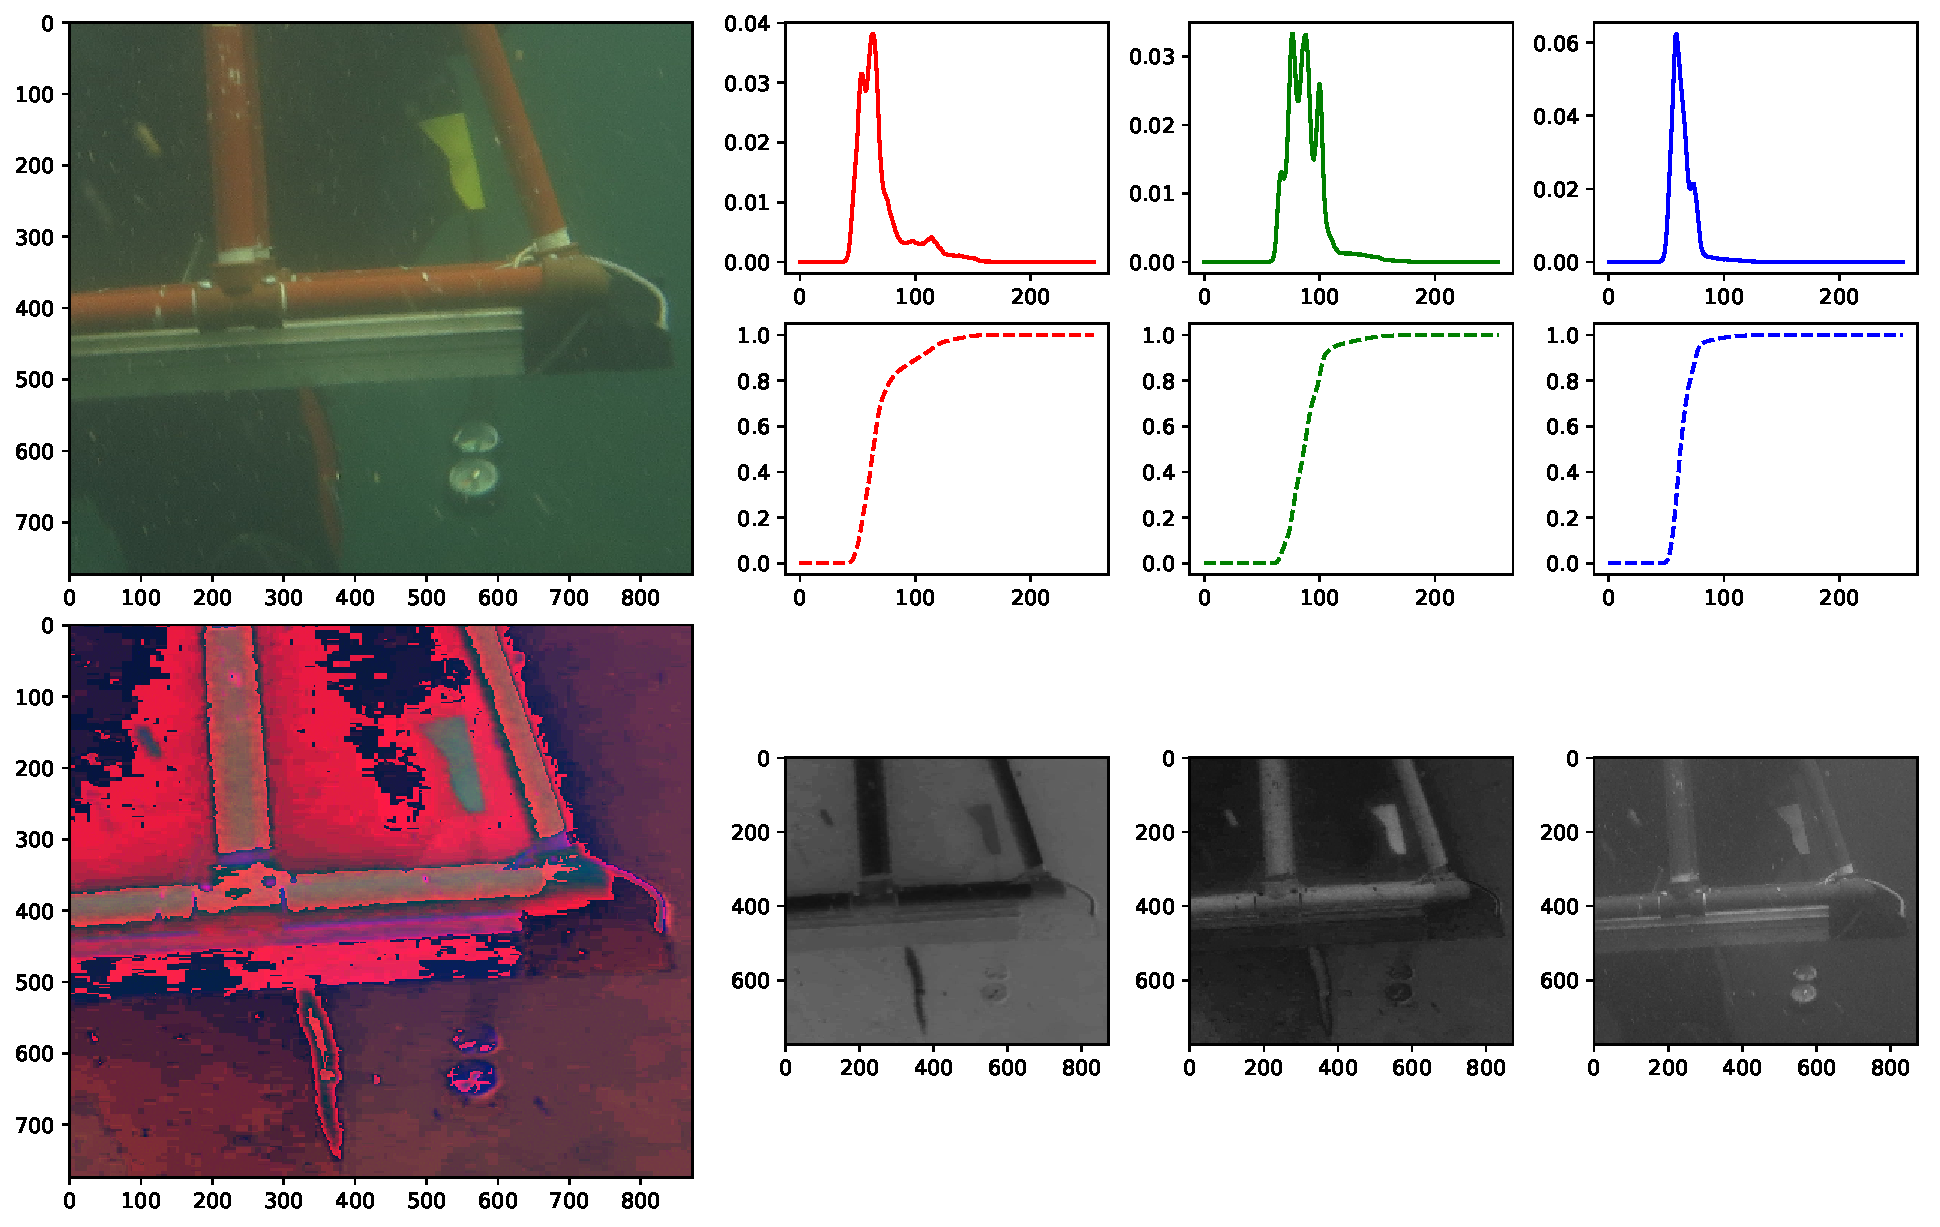
\includegraphics[height=6cm]{informe-imgs/ej01-c-1.pdf}
  \caption{\texttt{python3 practica1/ej01-c.py test/imagenesClaseColor/1907xx.png}}
\end{figure}
\begin{figure}[H]
\centering
  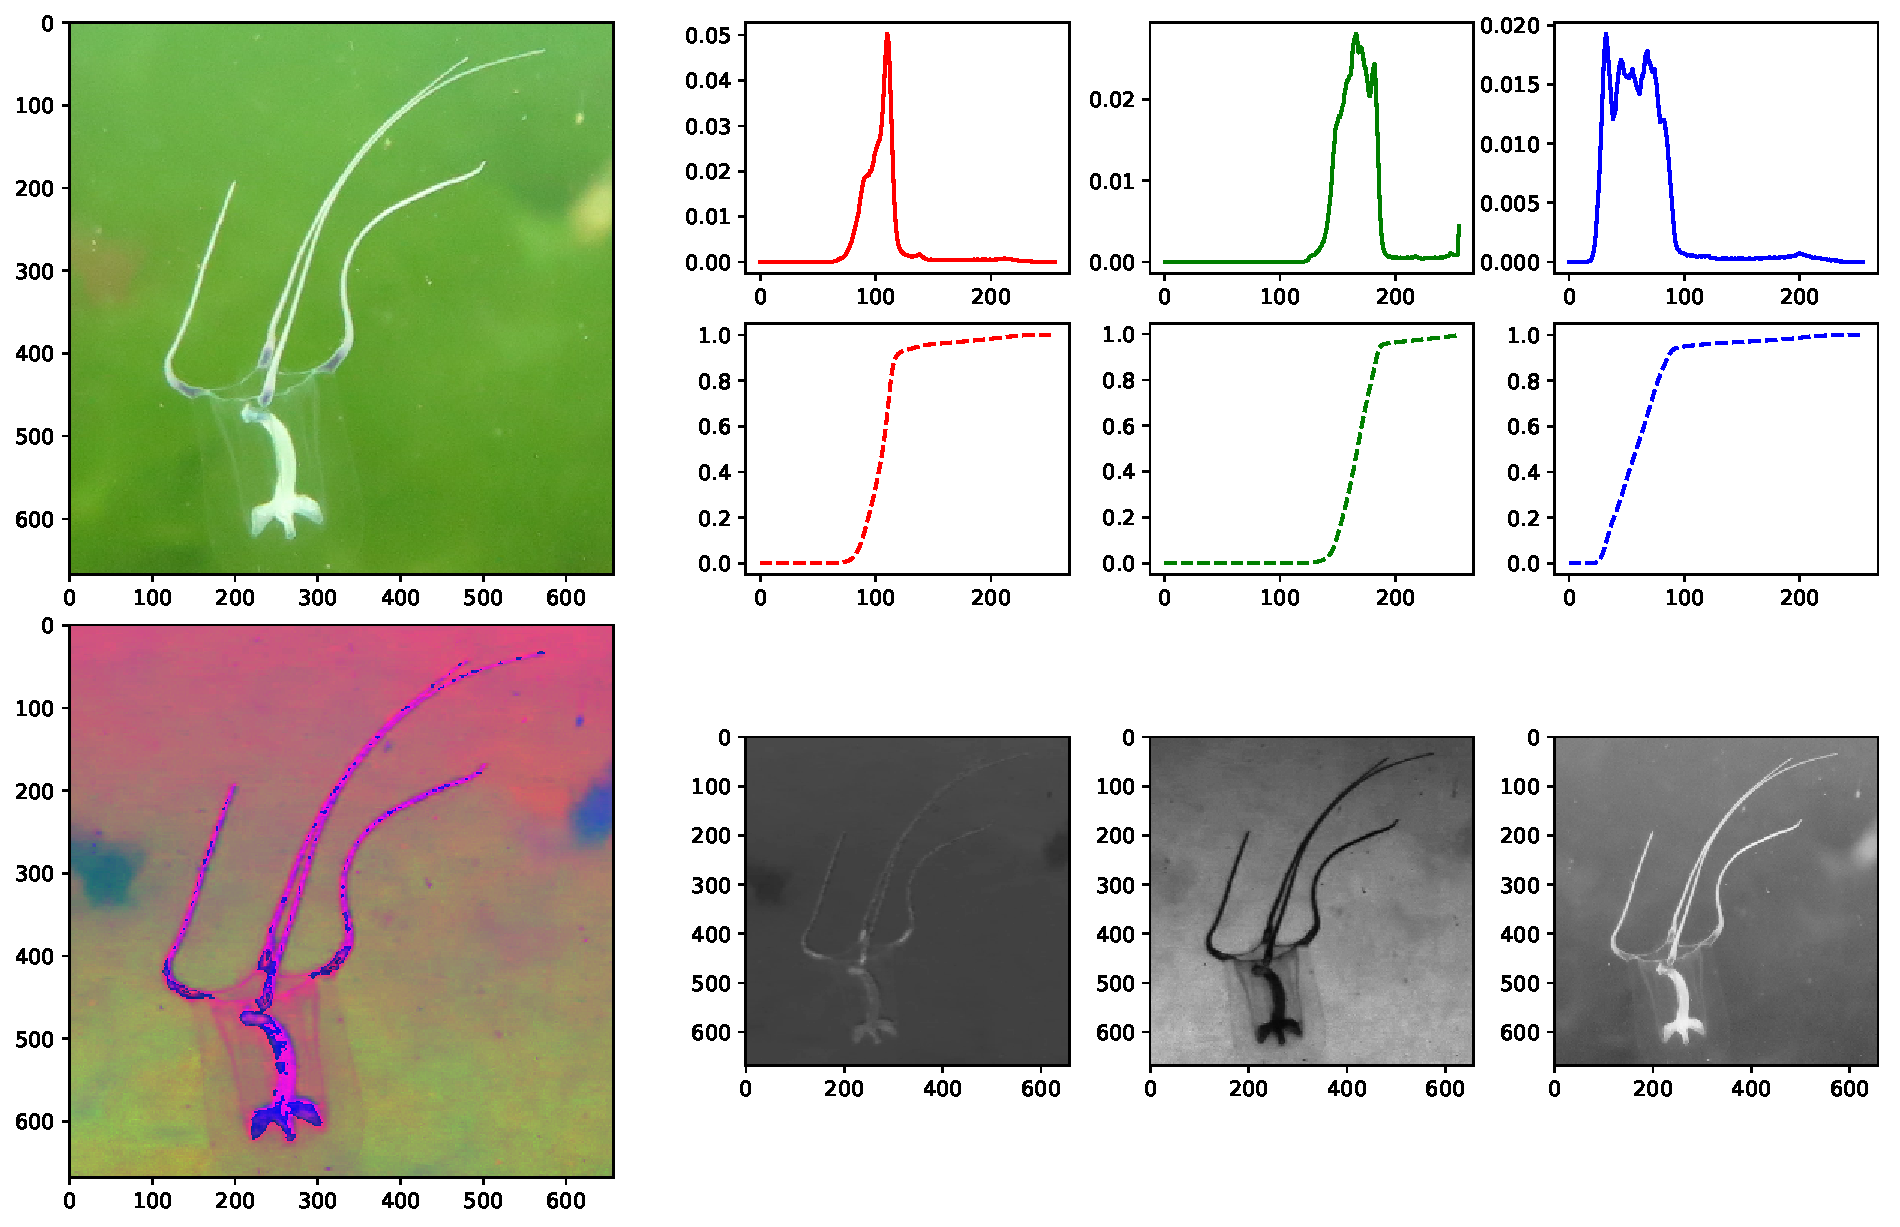
\includegraphics[height=6cm]{informe-imgs/ej01-c-2.pdf}
  \caption{\texttt{python3 practica1/ej01-c.py test/imagenesClaseColor/1901xx.png}}
\end{figure}

\subsection{Ejercicio 1.d.}

Ecualización del canal I.

Modo de uso
\begin{verbatim}
    python3 ej01-d.py <img>
\end{verbatim}

\subsubsection*{Ejemplos}
\begin{figure}[H]
\centering
  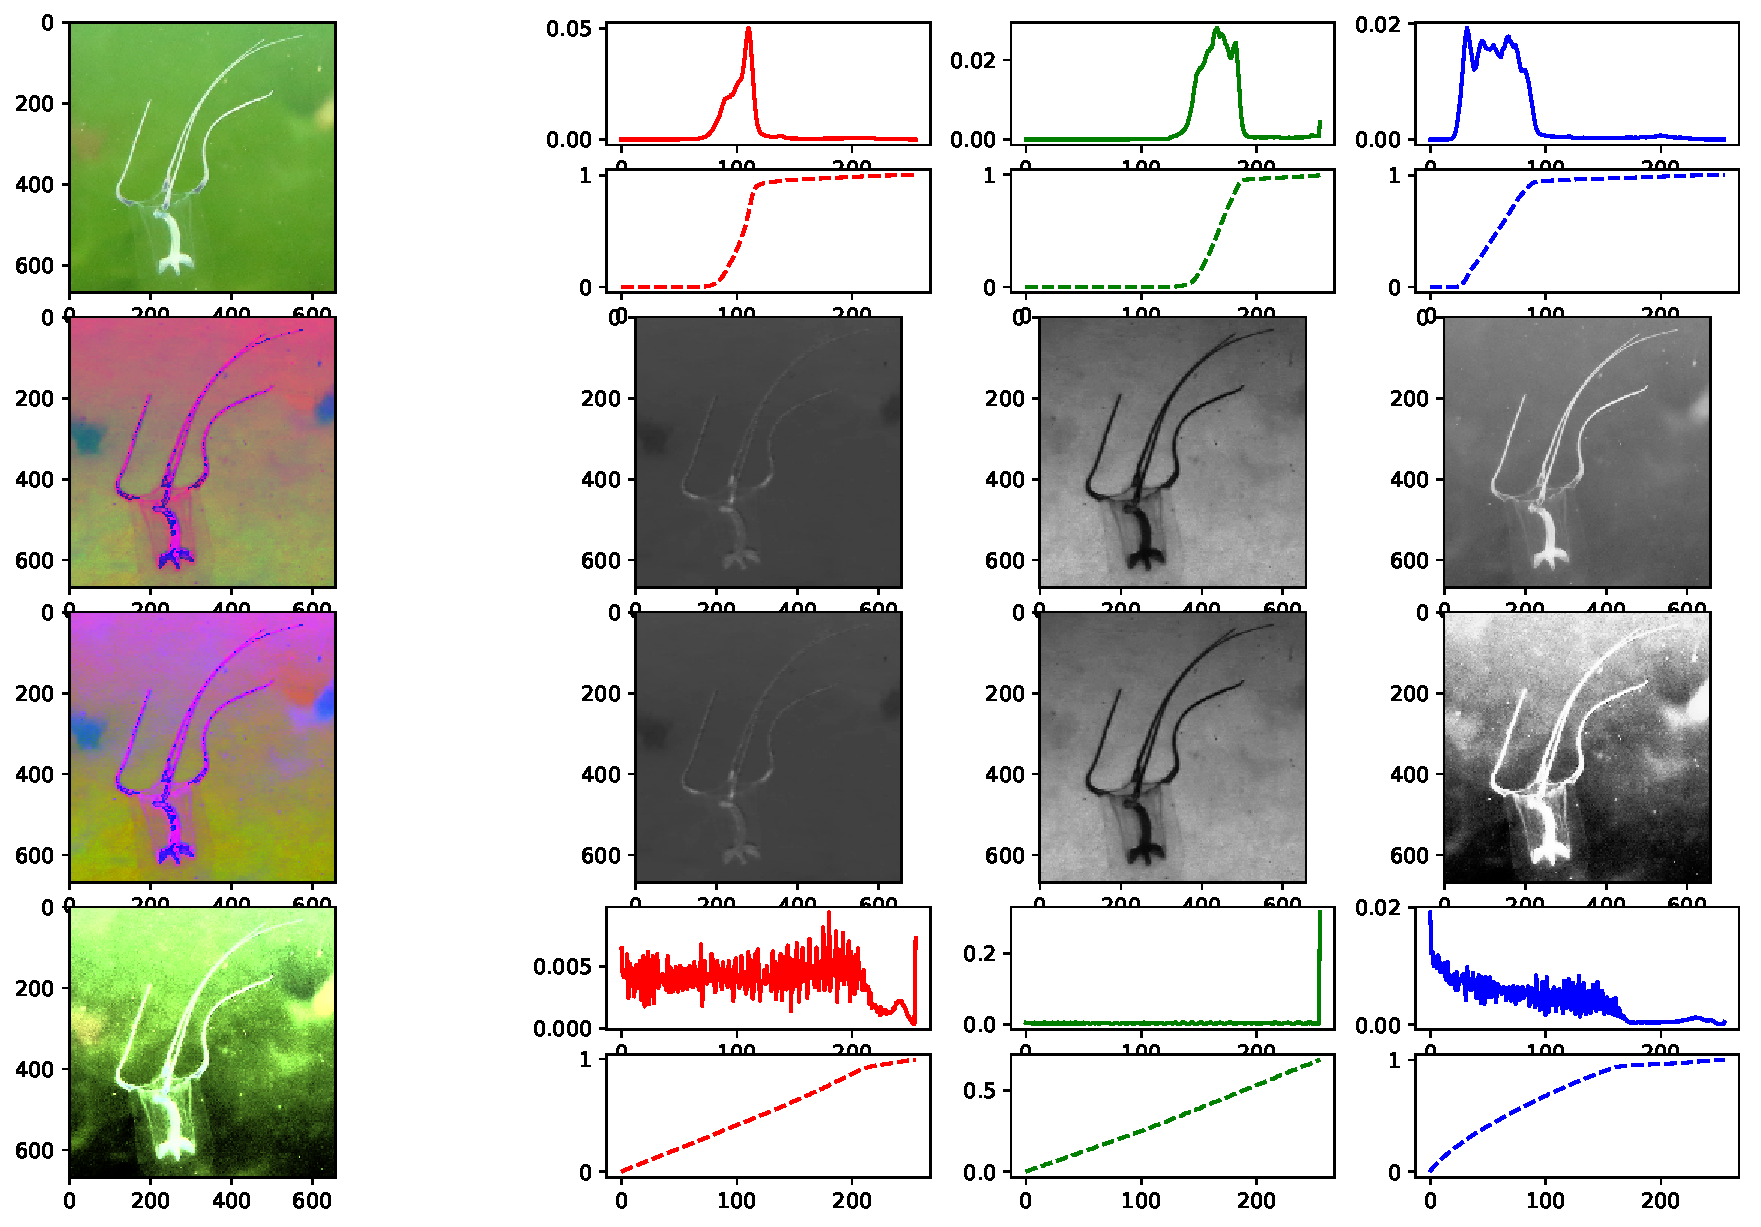
\includegraphics[height=6cm]{informe-imgs/ej01-d-1.pdf}
  \caption{\texttt{python3 practica1/ej01-d.py test/imagenesClaseColor/1901xx.png}}
\end{figure}
\begin{figure}[H]
\centering
  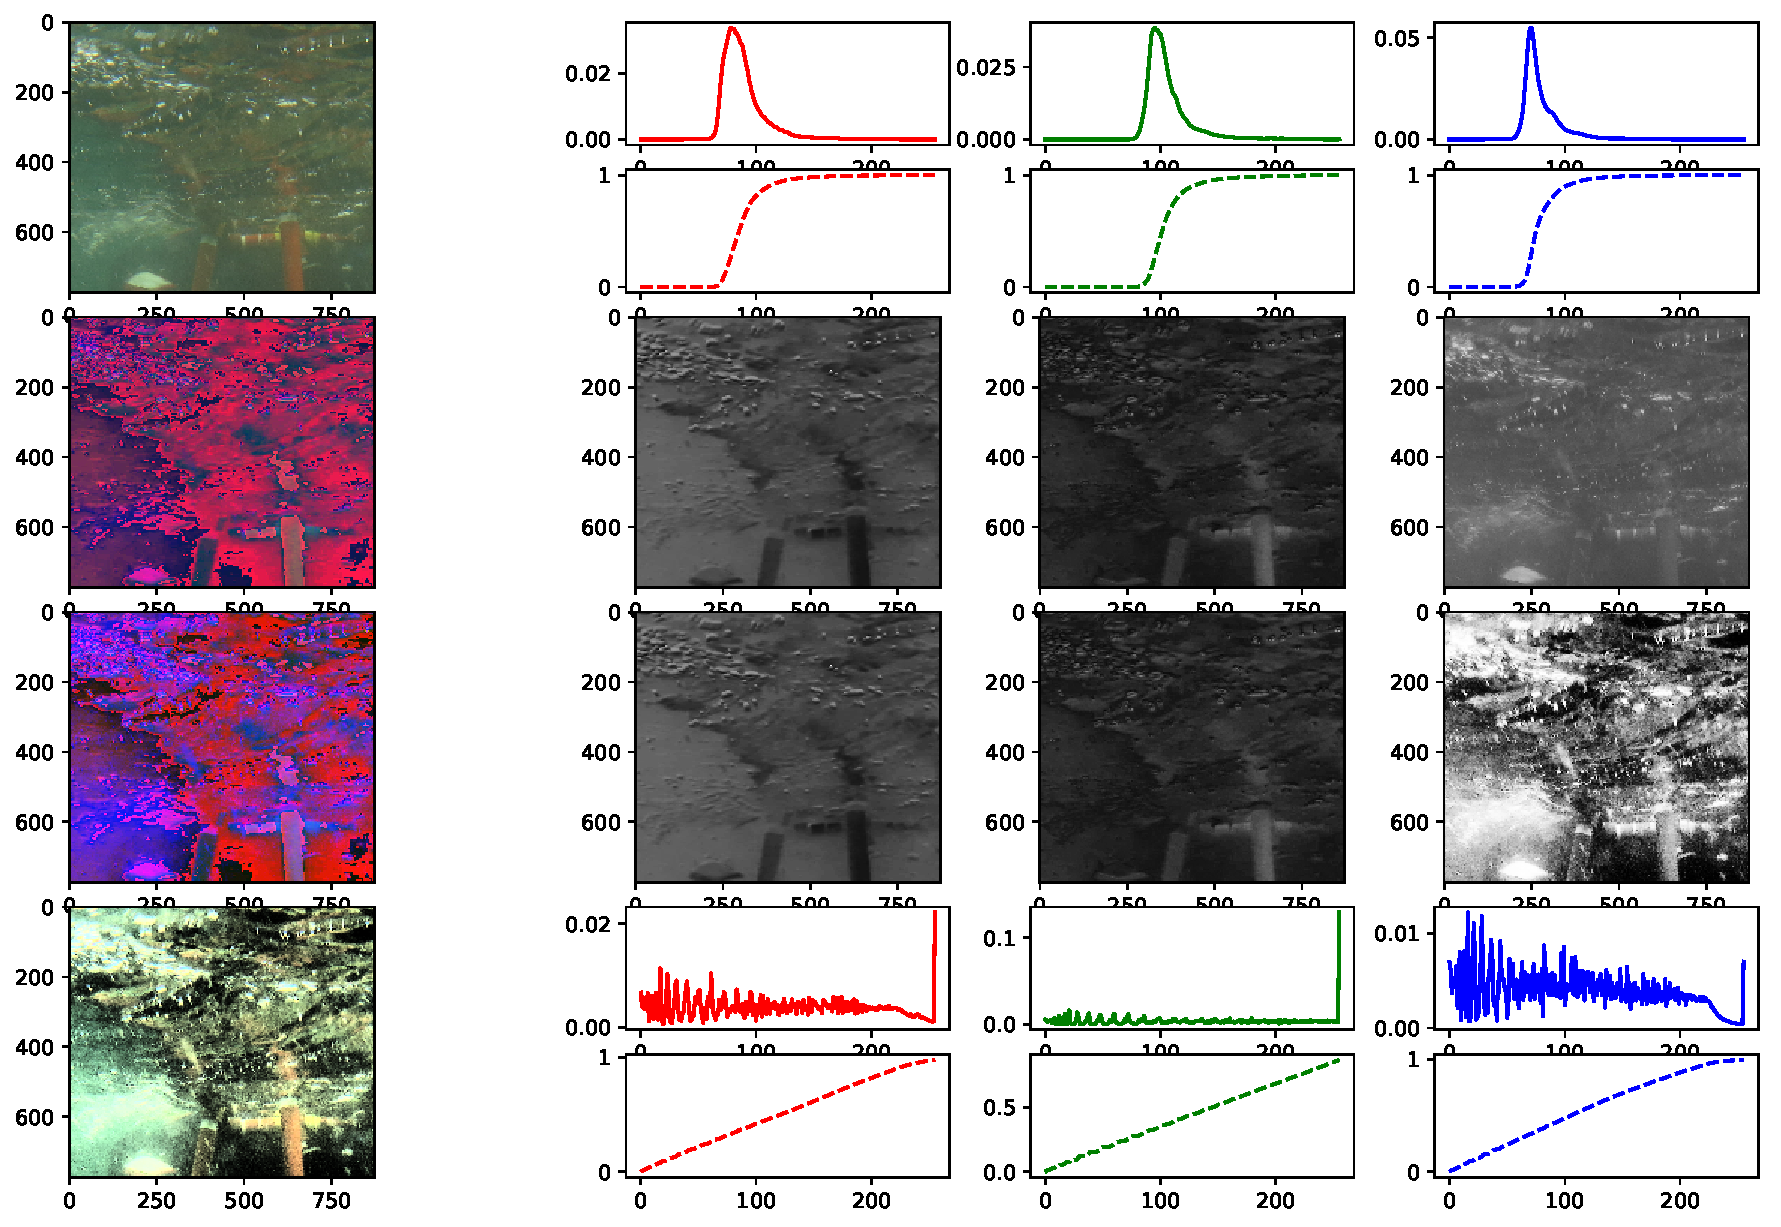
\includegraphics[height=6cm]{informe-imgs/ej01-d-2.pdf}
  \caption{\texttt{python3 practica1/ej01-d.py test/imagenesClaseColor/1908iv.png}}
\end{figure}
\begin{figure}[H]
\centering
  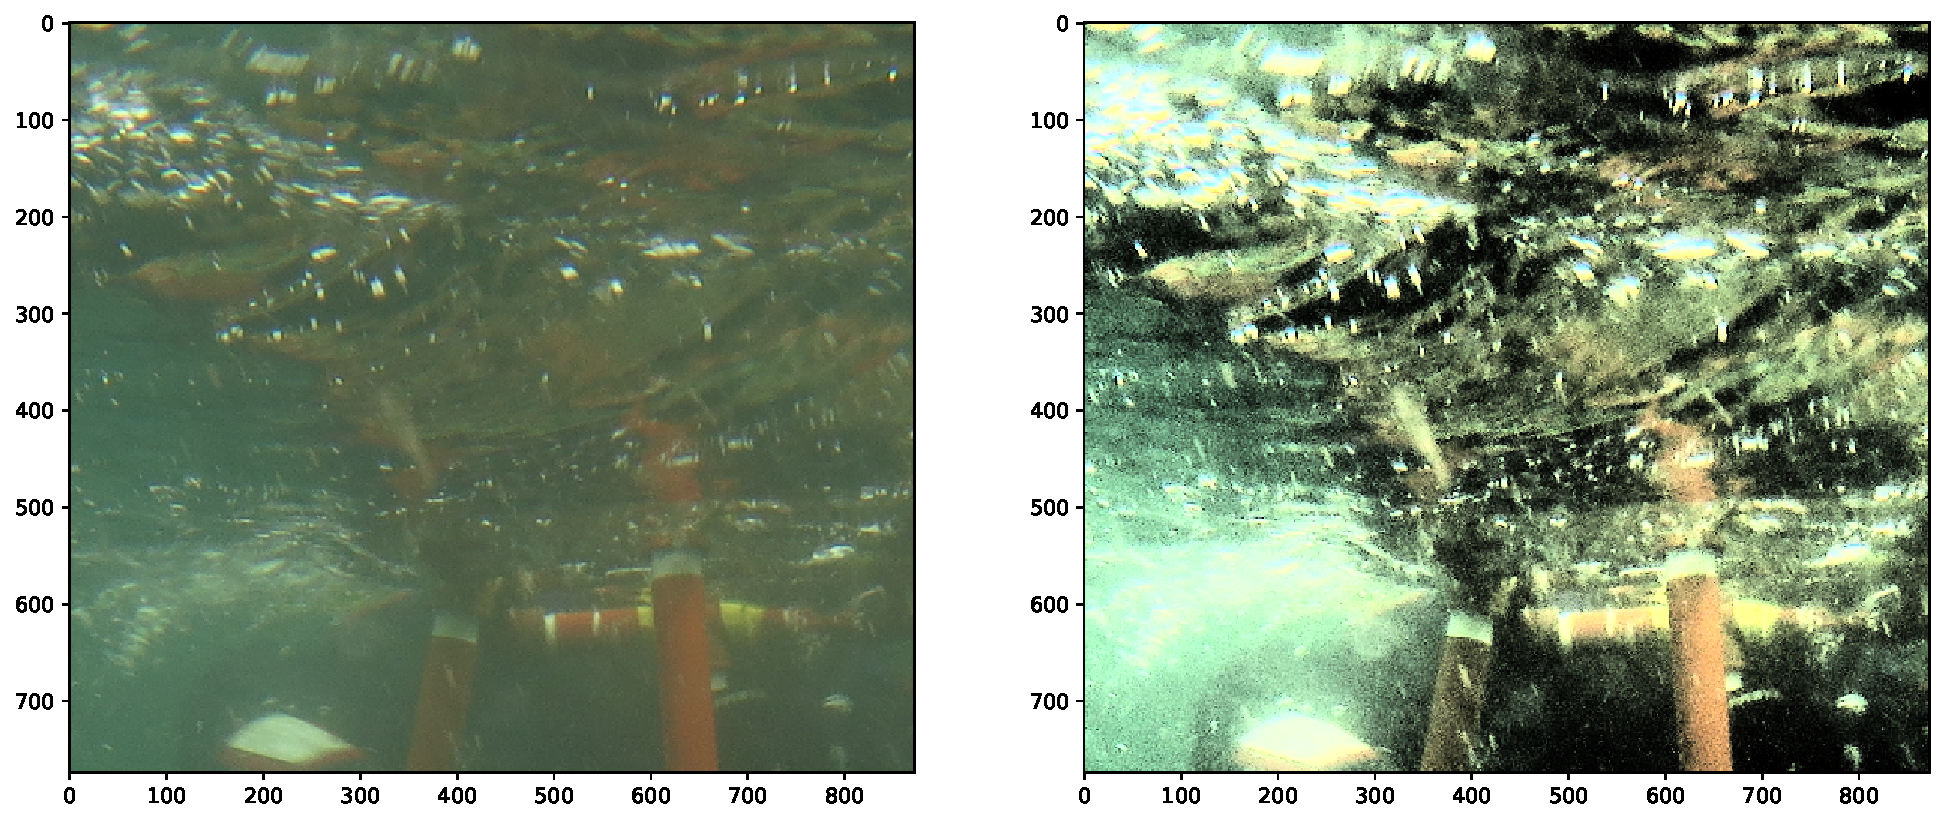
\includegraphics[height=6cm]{informe-imgs/ej01-d-3.pdf}
  \caption{\texttt{python3 practica1/ej01-d.py test/imagenesClaseColor/1908iv.png}}
\end{figure}

\subsection{Ejercicio 1.e.}

Diferentes transformaciones puntuales.

Modo de uso
\begin{verbatim}
    python3 ej01-e.py <img>   # Cambiando el codigo a mano para usar el filtro deseado.
\end{verbatim}

\subsubsection*{Ejemplos}
Transformación logaritmica al canal I.
\begin{figure}[H]
\centering
  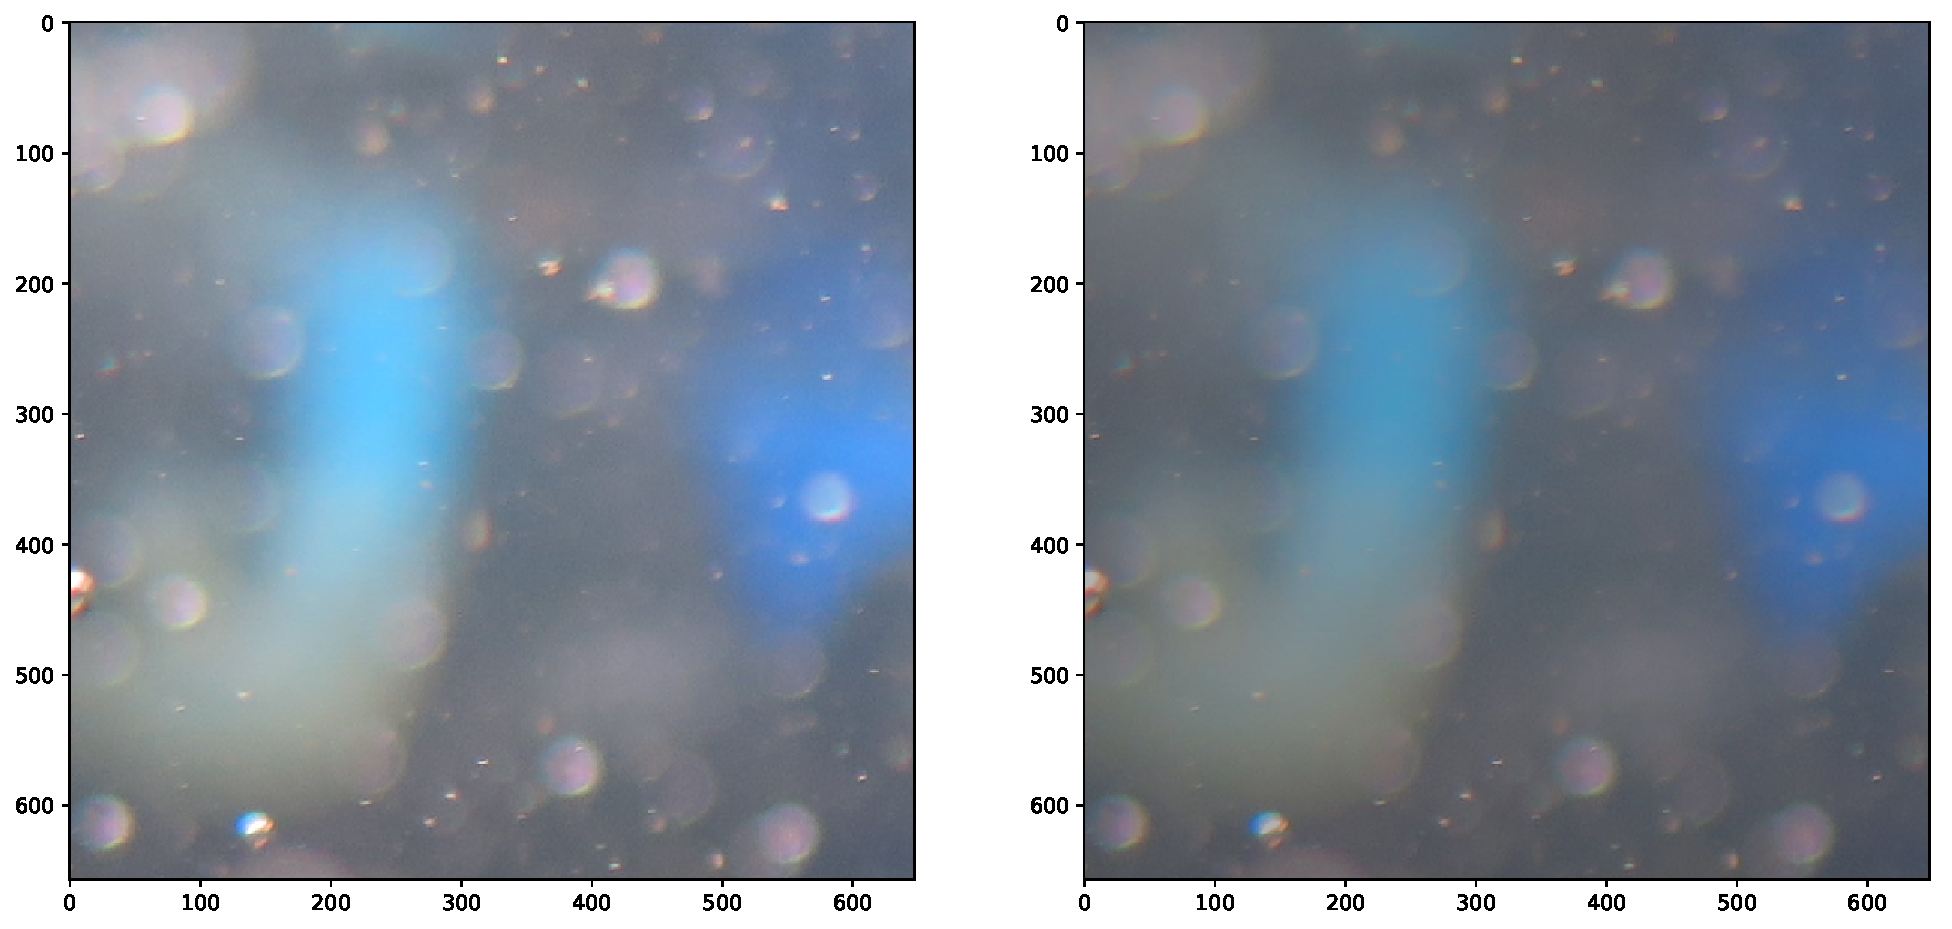
\includegraphics[height=6cm]{informe-imgs/ej01-e-1.pdf}
  \caption{\texttt{python3 practica1/ej01-e.py test/imagenesClaseColor/1923xx.png}}
\end{figure}

Transformación logaritmica al canal S.
\begin{figure}[H]
\centering
  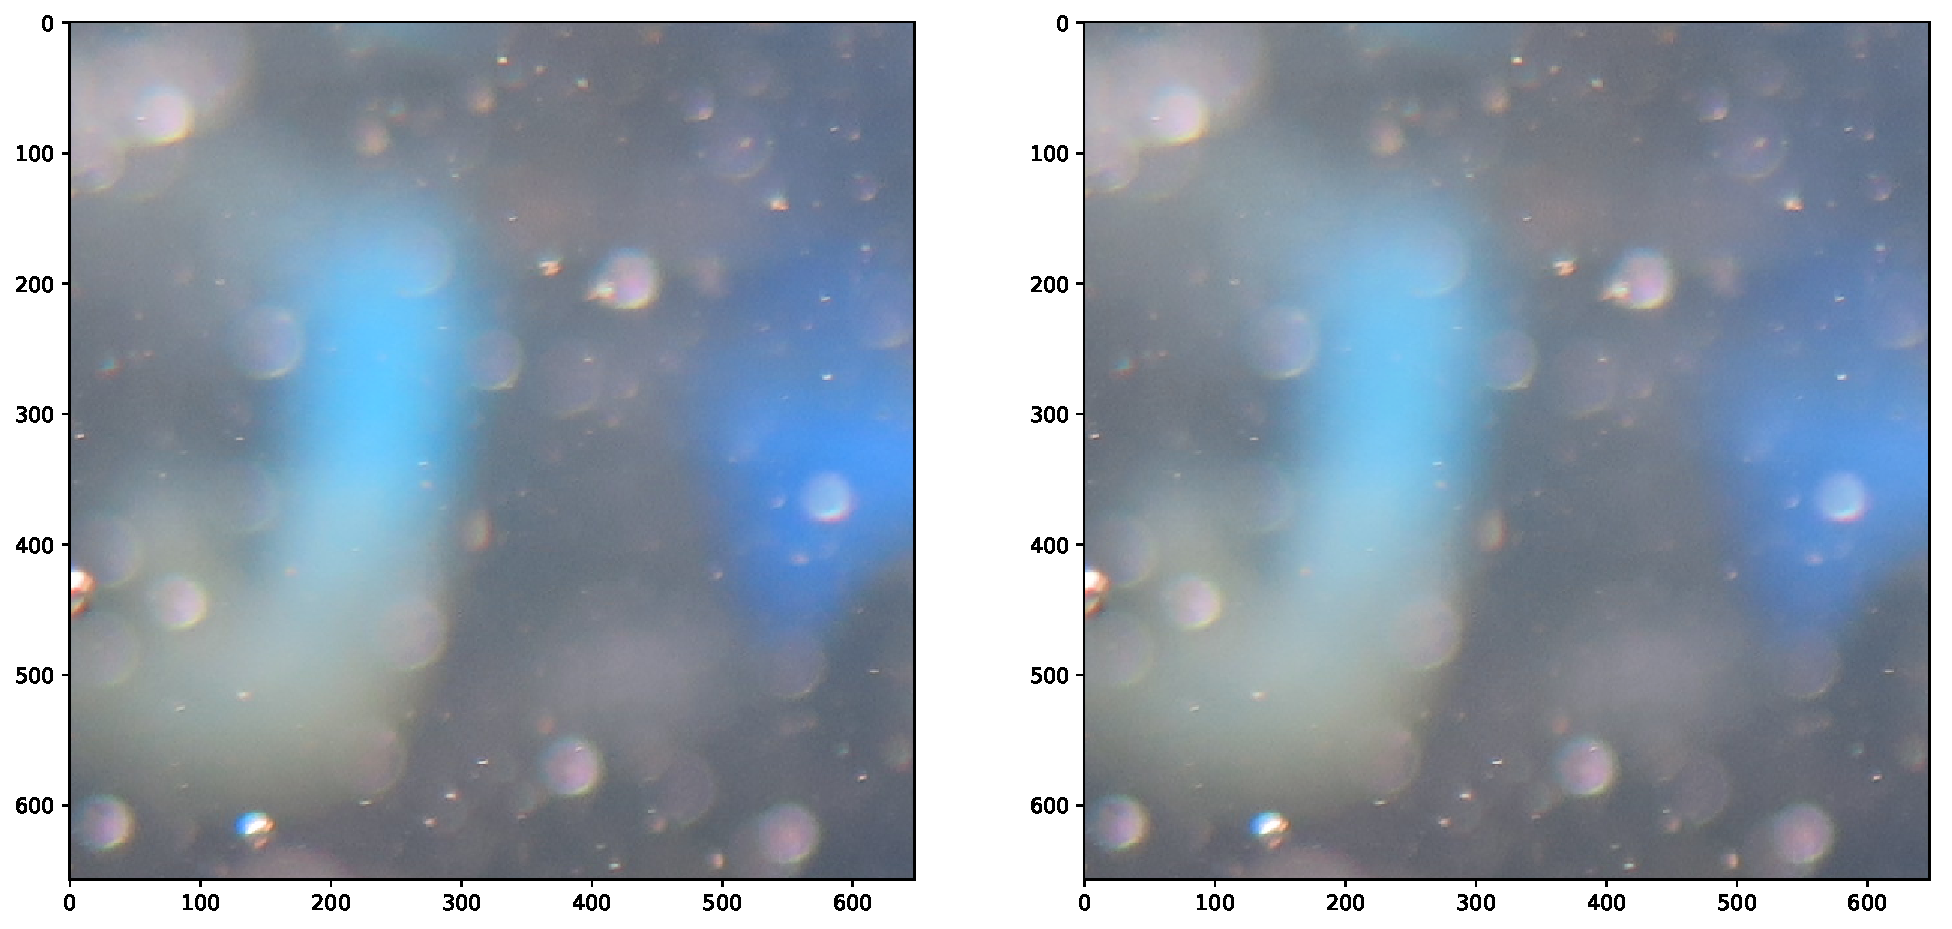
\includegraphics[height=6cm]{informe-imgs/ej01-e-2.pdf}
  \caption{\texttt{python3 practica1/ej01-e.py test/imagenesClaseColor/1923xx.png}}
\end{figure}

Intercambio de canales S e I.
\begin{figure}[H]
\centering
  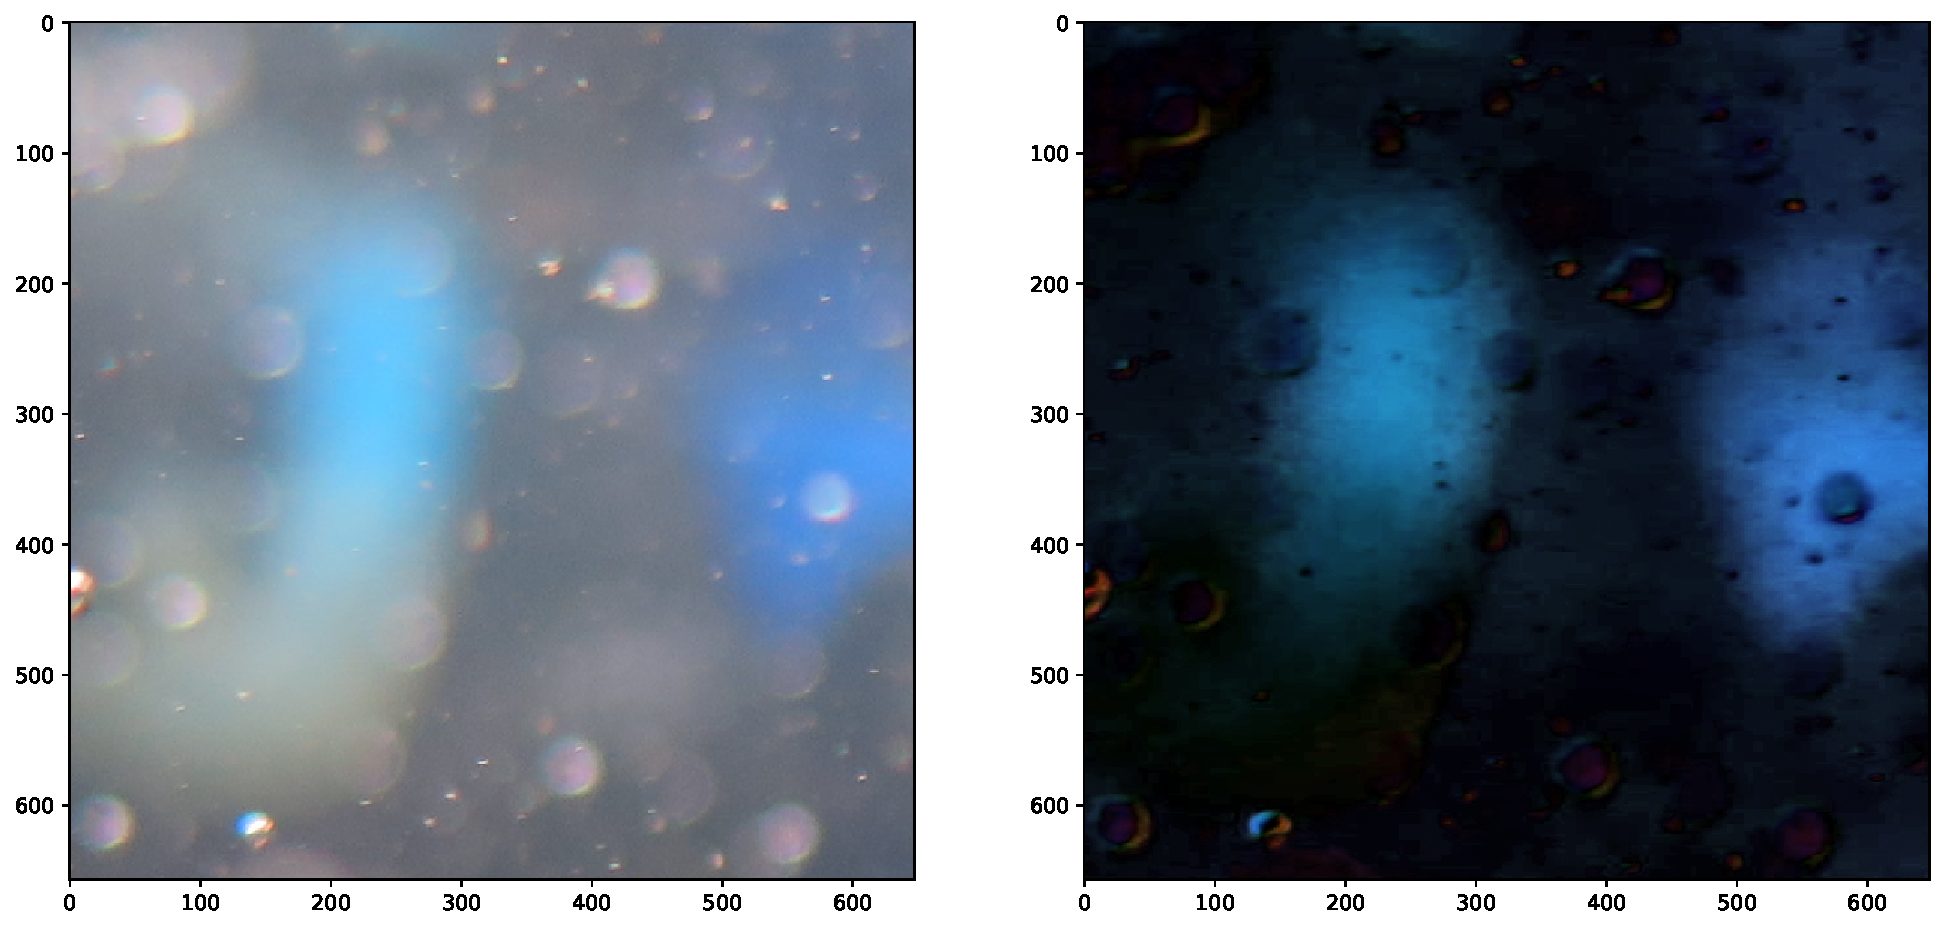
\includegraphics[height=6cm]{informe-imgs/ej01-e-3.pdf}
  \caption{\texttt{python3 practica1/ej01-e.py test/imagenesClaseColor/1923xx.png}}
\end{figure}

\newpage

\section{Ejercicio 2.}
\subsection{Ejercicio 2.a.}

Realce de saturación.

Modo de uso
\begin{verbatim}
    python3 ej02-a.py <img> <c>
\end{verbatim}

\subsection*{Ejemplos}
$c = 4$
\begin{figure}[H]
\centering
  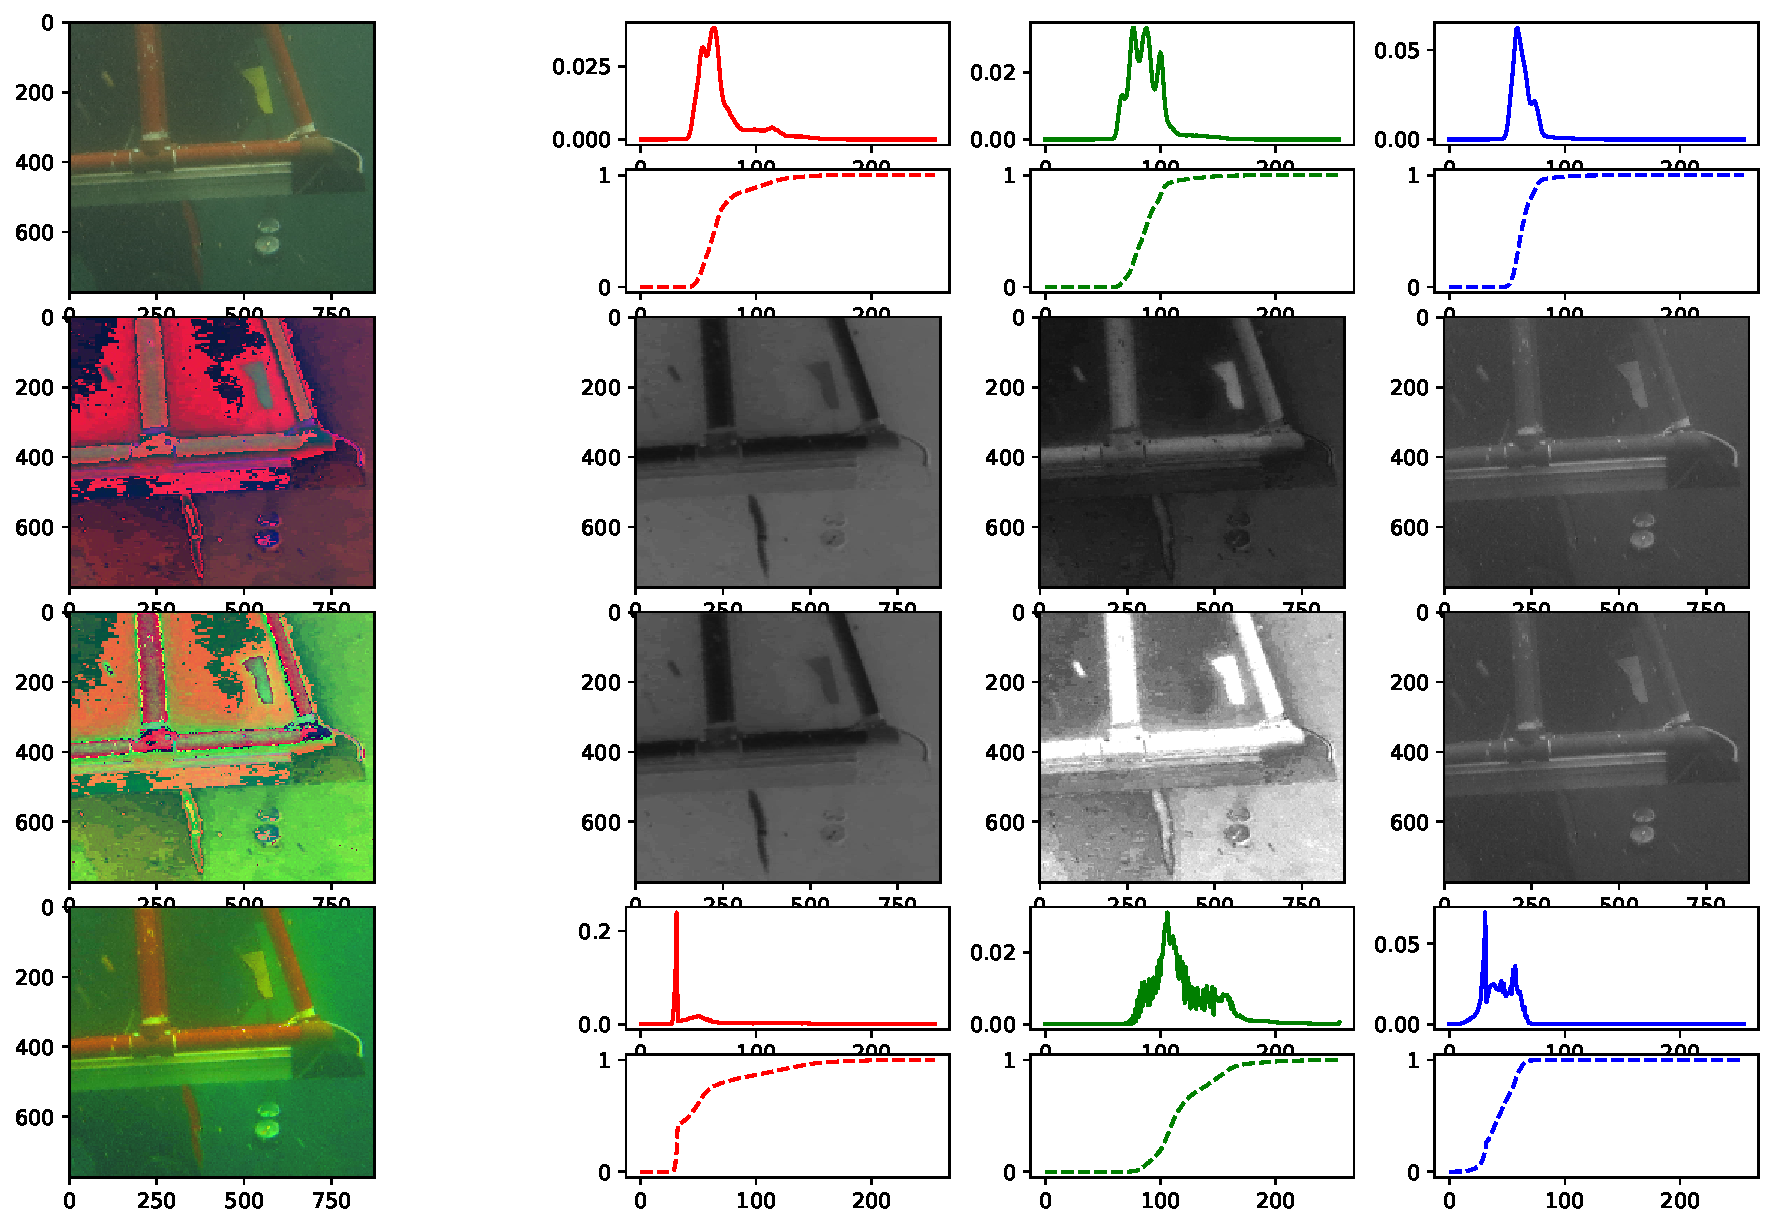
\includegraphics[height=6cm]{informe-imgs/ej02-a-1.pdf}
  \caption{\texttt{python3 practica1/ej02-a.py test/imagenesClaseColor/1907xx.png 4}}
\end{figure}
\begin{figure}[H]
\centering
  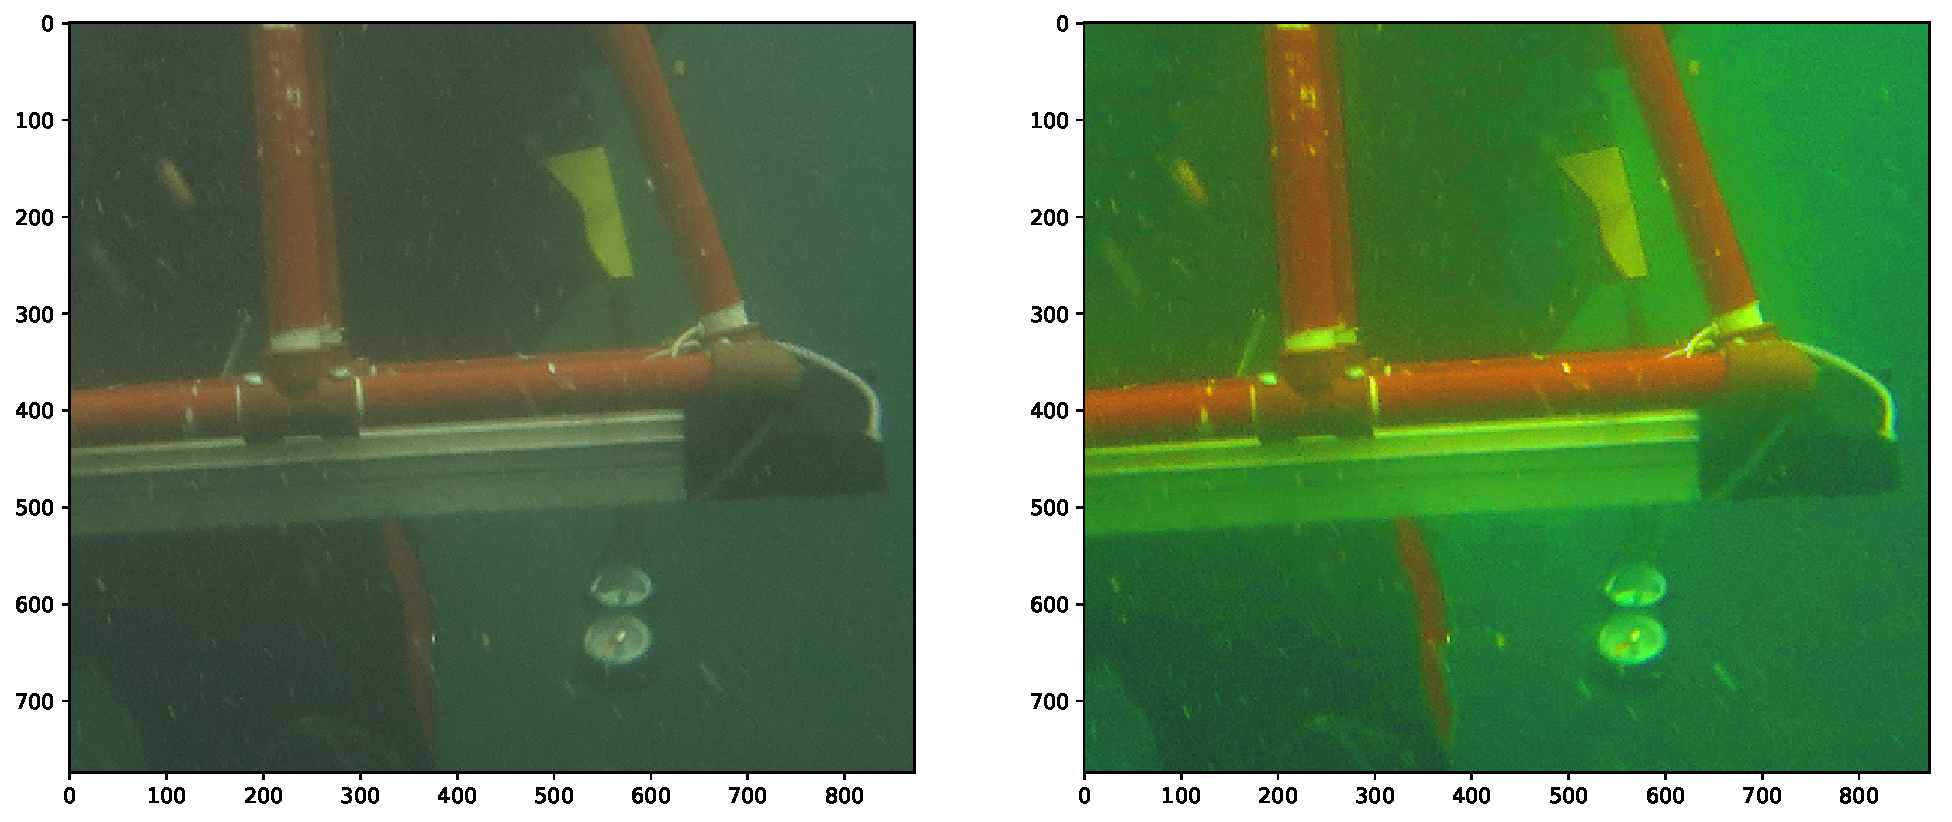
\includegraphics[height=6cm]{informe-imgs/ej02-a-2.pdf}
  \caption{\texttt{python3 practica1/ej02-a.py test/imagenesClaseColor/1907xx.png 4 --end}}
\end{figure}

$c = 0.5$
\begin{figure}[H]
\centering
  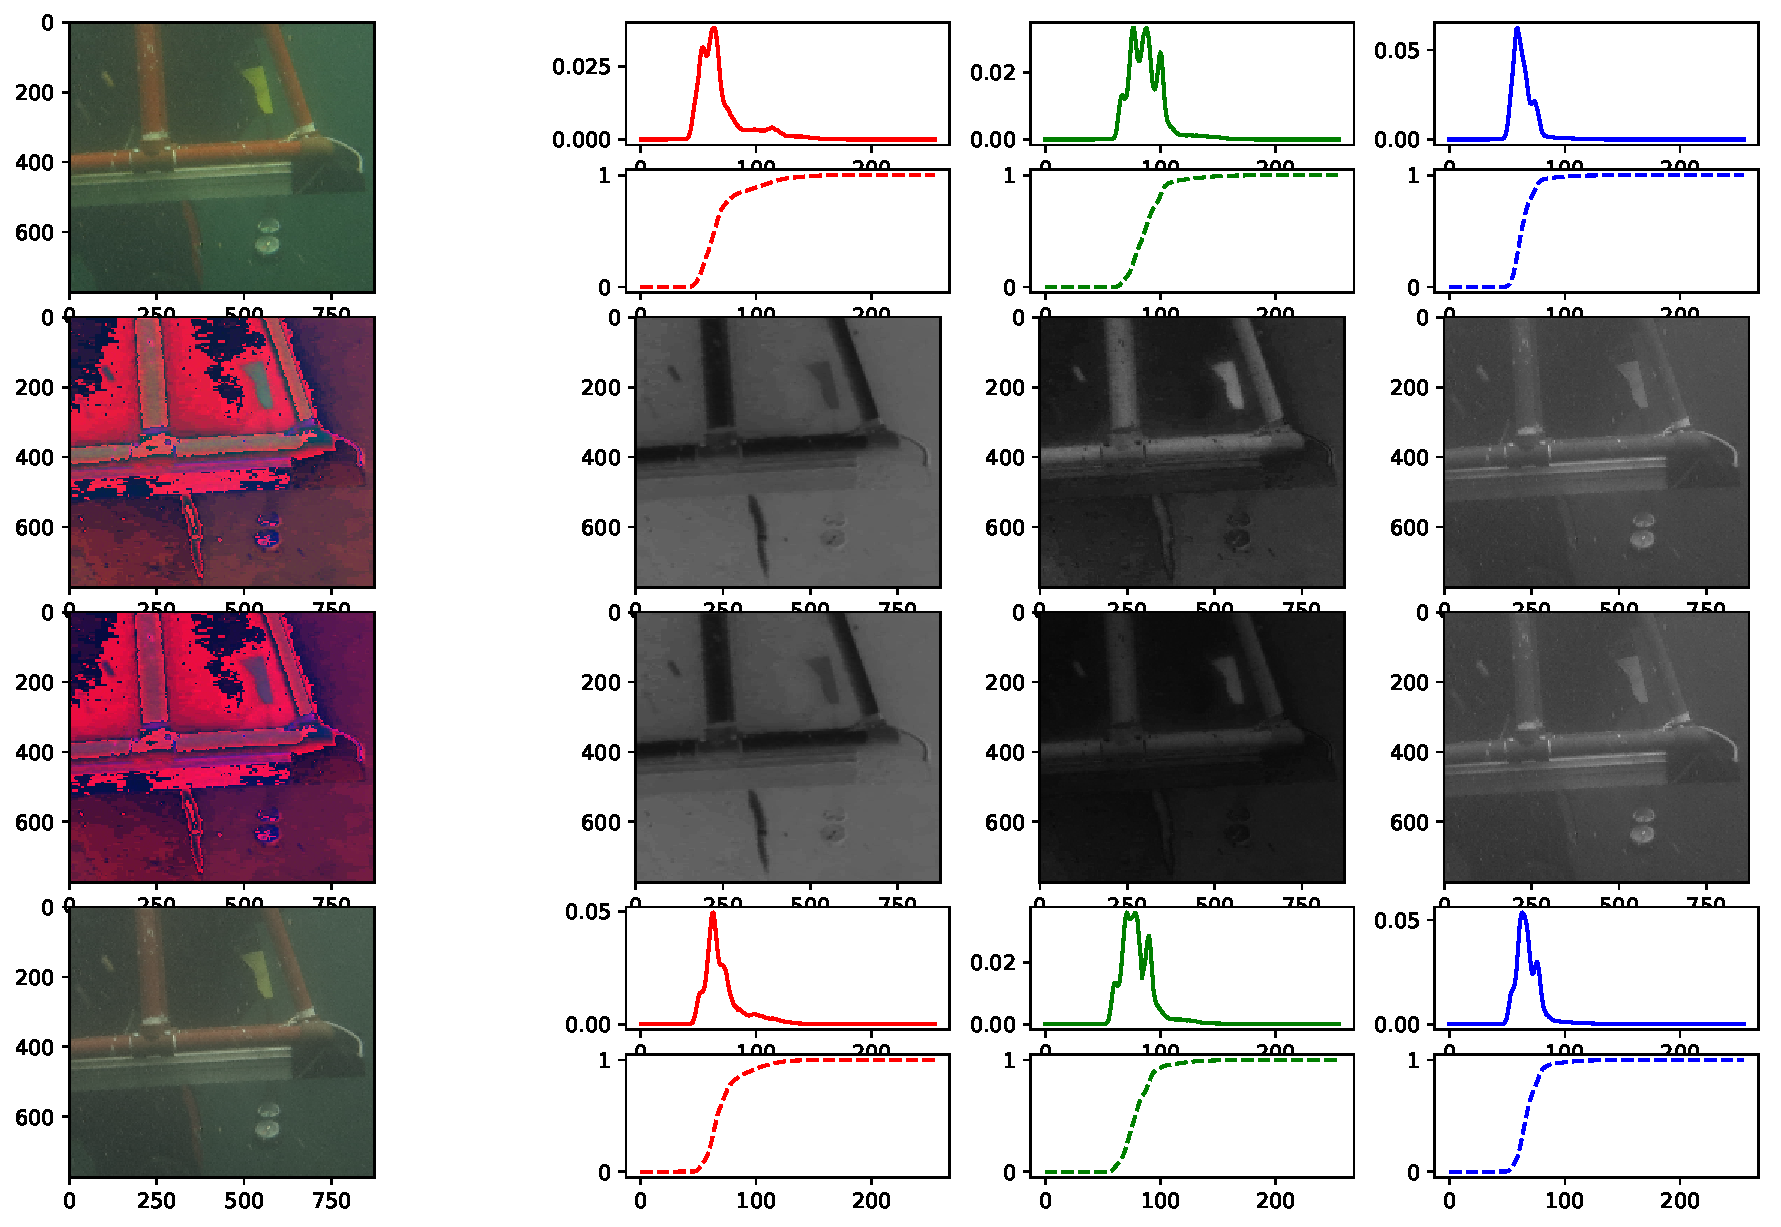
\includegraphics[height=6cm]{informe-imgs/ej02-a-3.pdf}
  \caption{\texttt{python3 practica1/ej02-a.py test/imagenesClaseColor/1907xx.png 0.5}}
\end{figure}

\begin{figure}[H]
\centering
  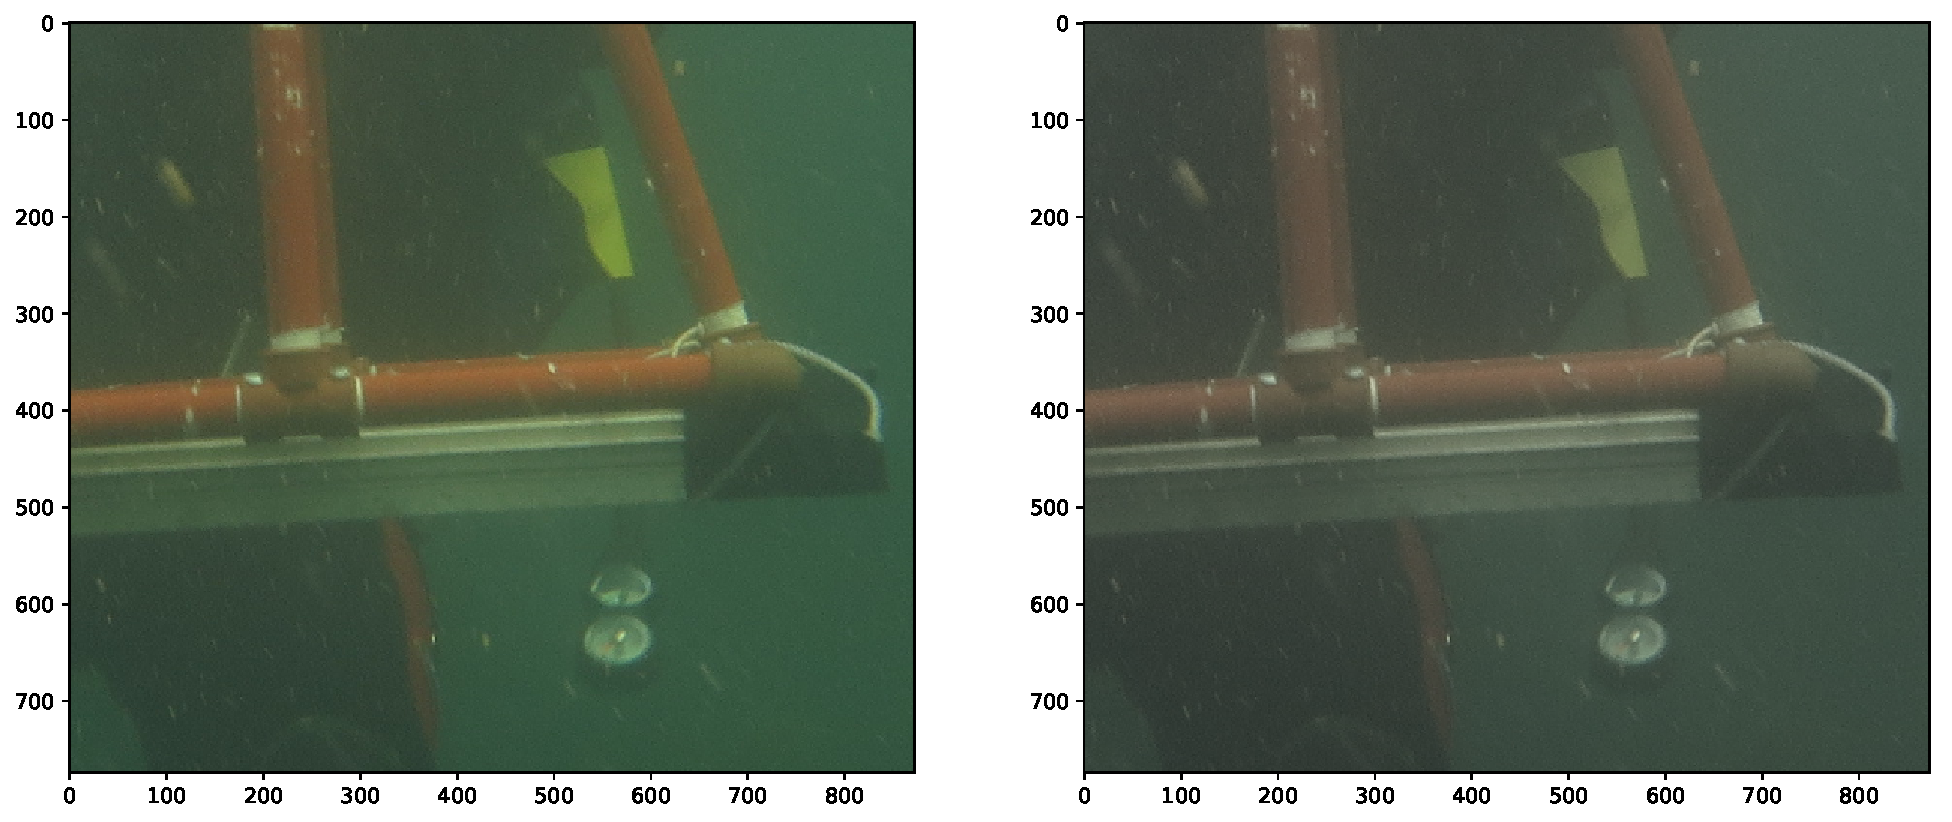
\includegraphics[height=6cm]{informe-imgs/ej02-a-4.pdf}
  \caption{\texttt{python3 practica1/ej02-a.py test/imagenesClaseColor/1907xx.png 0.5 --end}}
\end{figure}

\subsection{Ejercicio 2.b.}

Transformaciones variadas aplicadas al canal de saturación.

Modo de uso
\begin{verbatim}
    python3 ej02-b.py <img>    # Cambiando el codigo mandualmente para seleccionar el filtro.
\end{verbatim}

\subsubsection*{Ejemplos}

Umbral, valores mayores a $0.5$ van a $1$ y menores van a $0$.
\begin{figure}[H]
\centering
  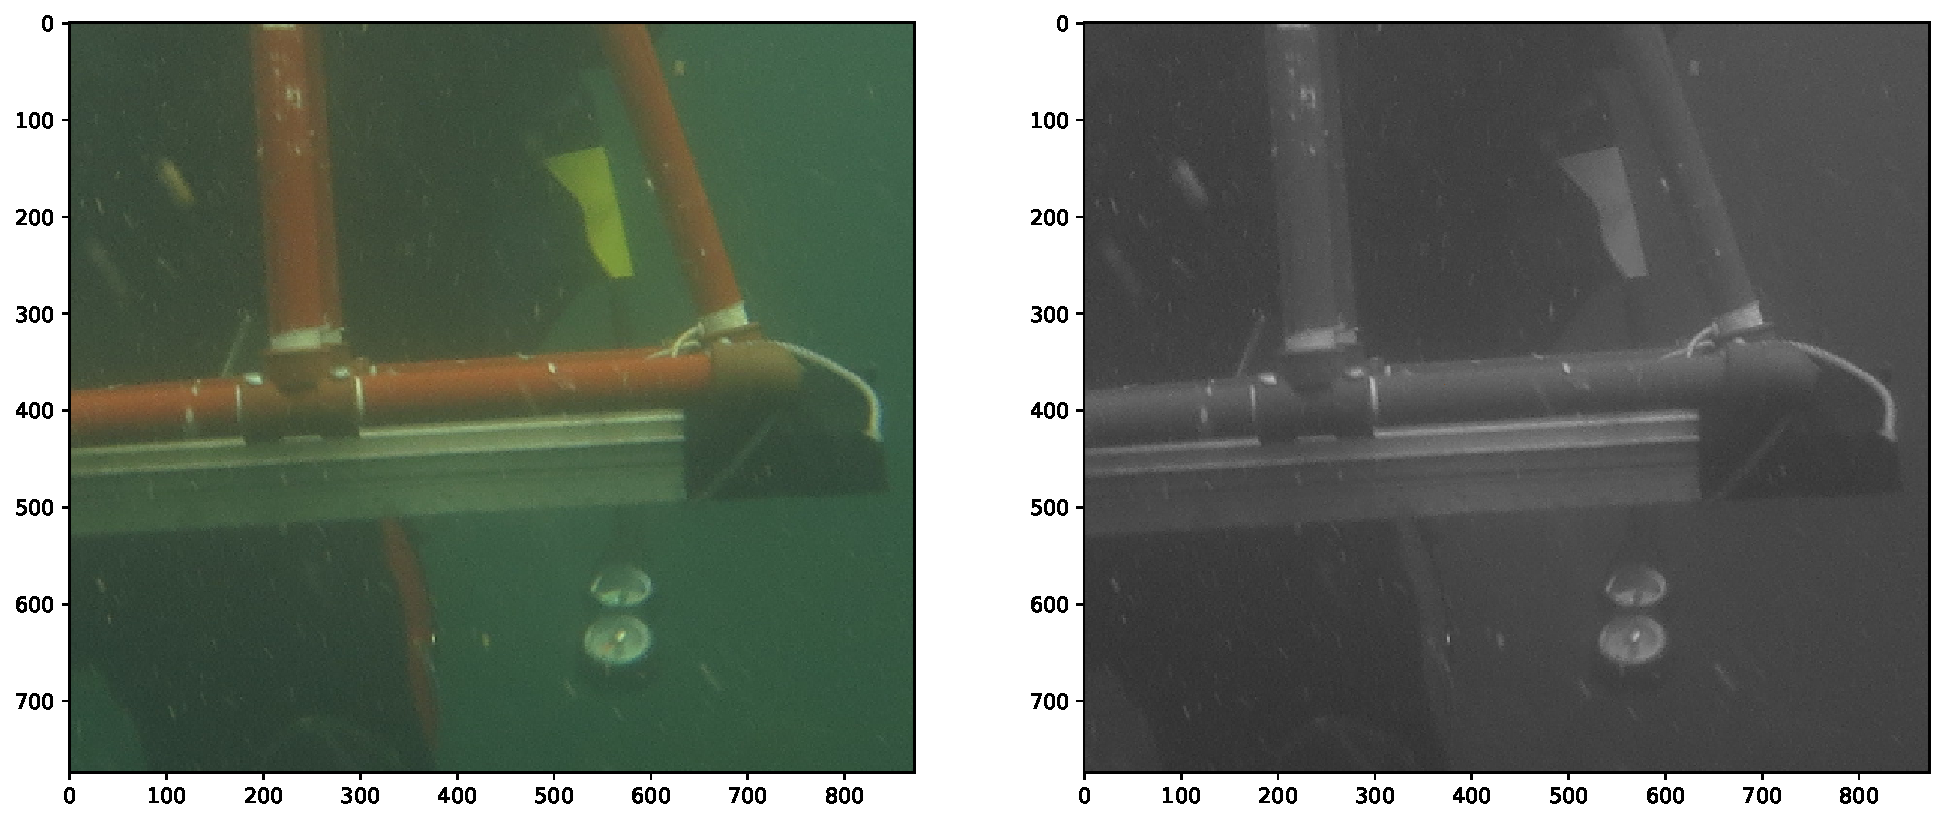
\includegraphics[height=6cm]{informe-imgs/ej02-b-1.pdf}
  \caption{\texttt{python3 practica1/ej02-b.py test/imagenesClaseColor/1907xx.png --end}}
\end{figure}

Ecualización del canal de saturación.
\begin{figure}[H]
\centering
  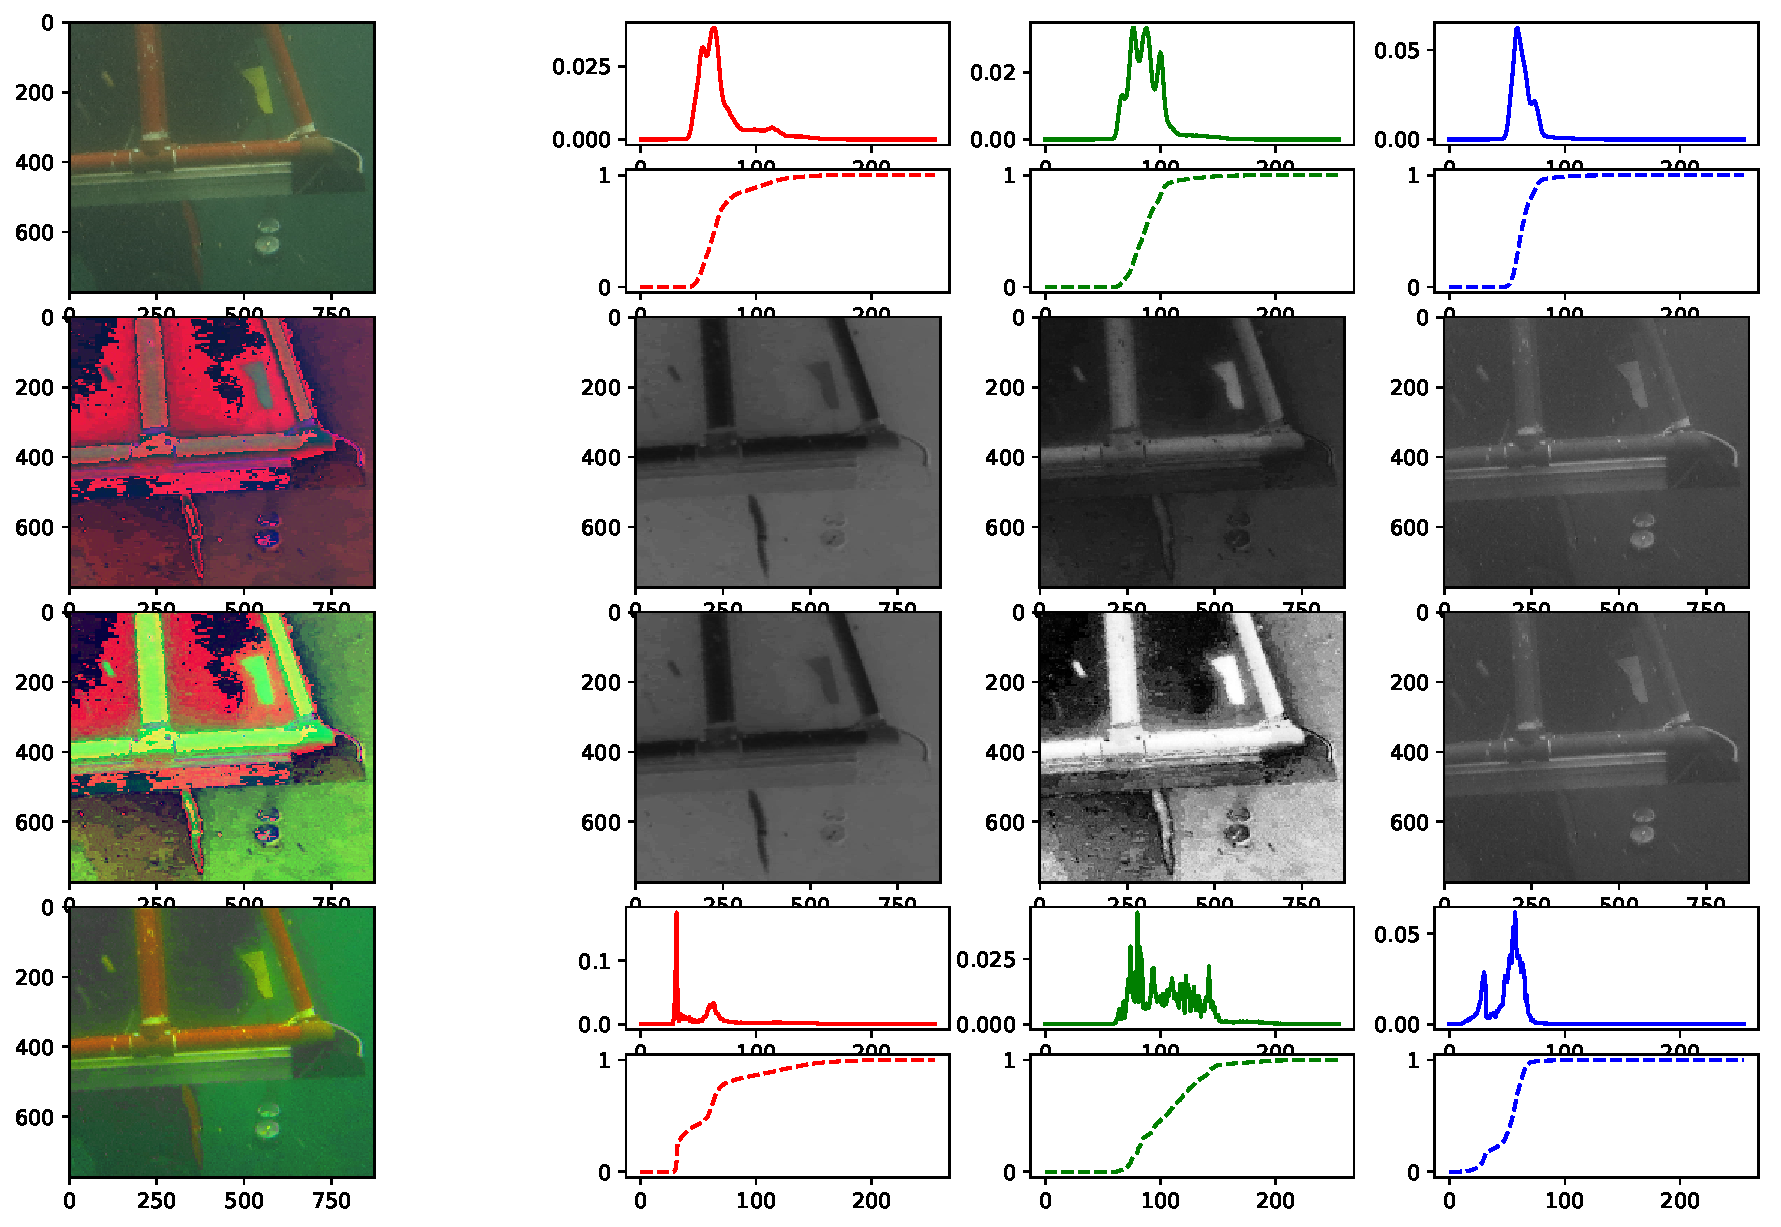
\includegraphics[height=6cm]{informe-imgs/ej02-b-2.pdf}
  \caption{\texttt{python3 practica1/ej02-b.py test/imagenesClaseColor/1907xx.png}}
\end{figure}
\begin{figure}[H]
\centering
  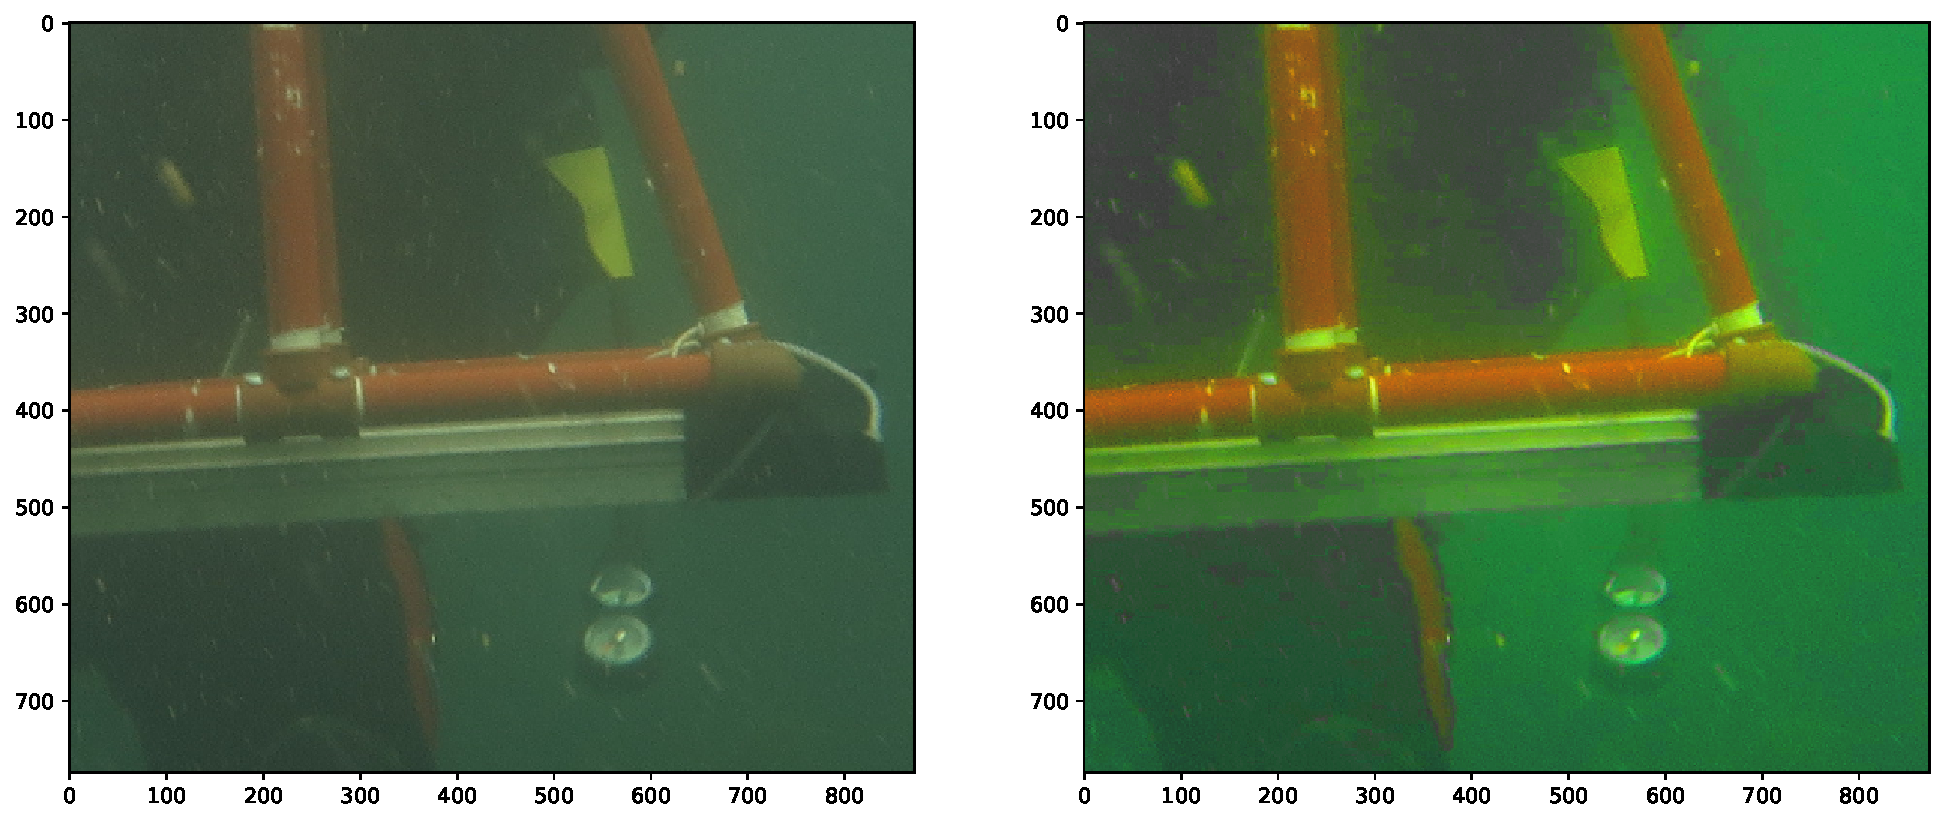
\includegraphics[height=6cm]{informe-imgs/ej02-b-3.pdf}
  \caption{\texttt{python3 practica1/ej02-b.py test/imagenesClaseColor/1907xx.png --end}}
\end{figure}

\newpage

\section{Ejercicio 3.}

Suma de constantes al valor de H.

Modo de uso
\begin{verbatim}
    python3 ej03-a.py <img> <c>
\end{verbatim}

\subsubsection*{Ejemplos}
\subsubsection*{Imagen 1 -- 1907xx}
$c = 0.5$
\begin{figure}[H]
\centering
  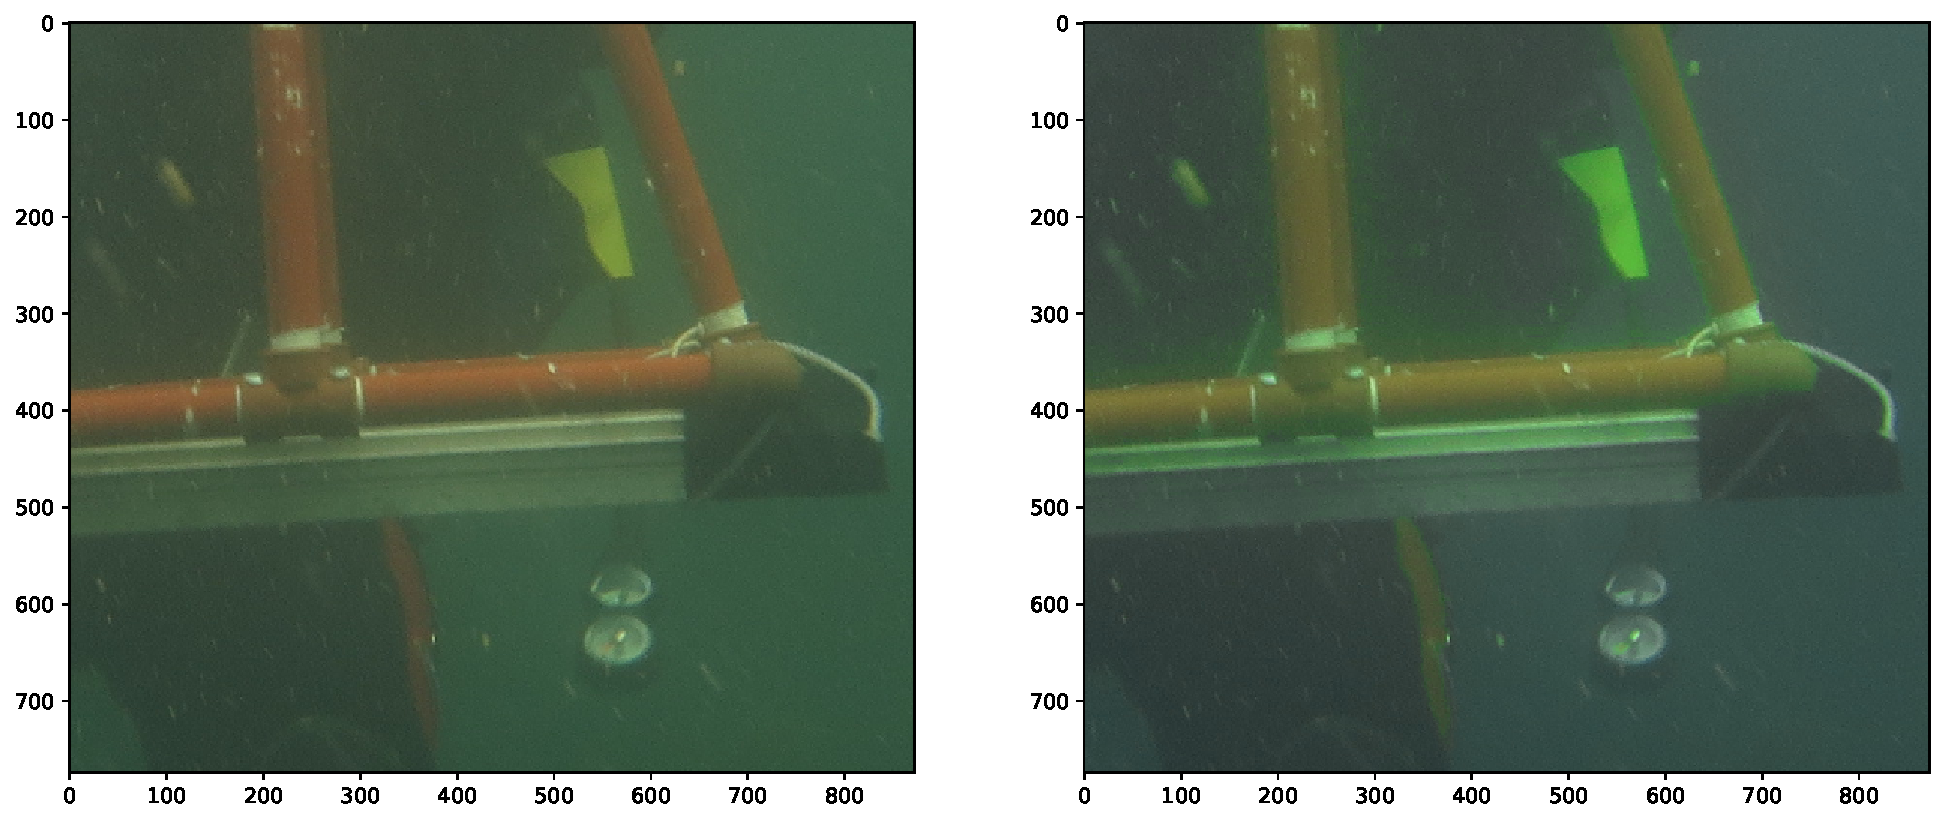
\includegraphics[height=6cm]{informe-imgs/ej03-1.pdf}
  \caption{\texttt{python3 practica1/ej03-a.py 0.5 test/imagenesClaseColor/1907xx.png --end}}
\end{figure}

$c = 2.5$
\begin{figure}[H]
\centering
  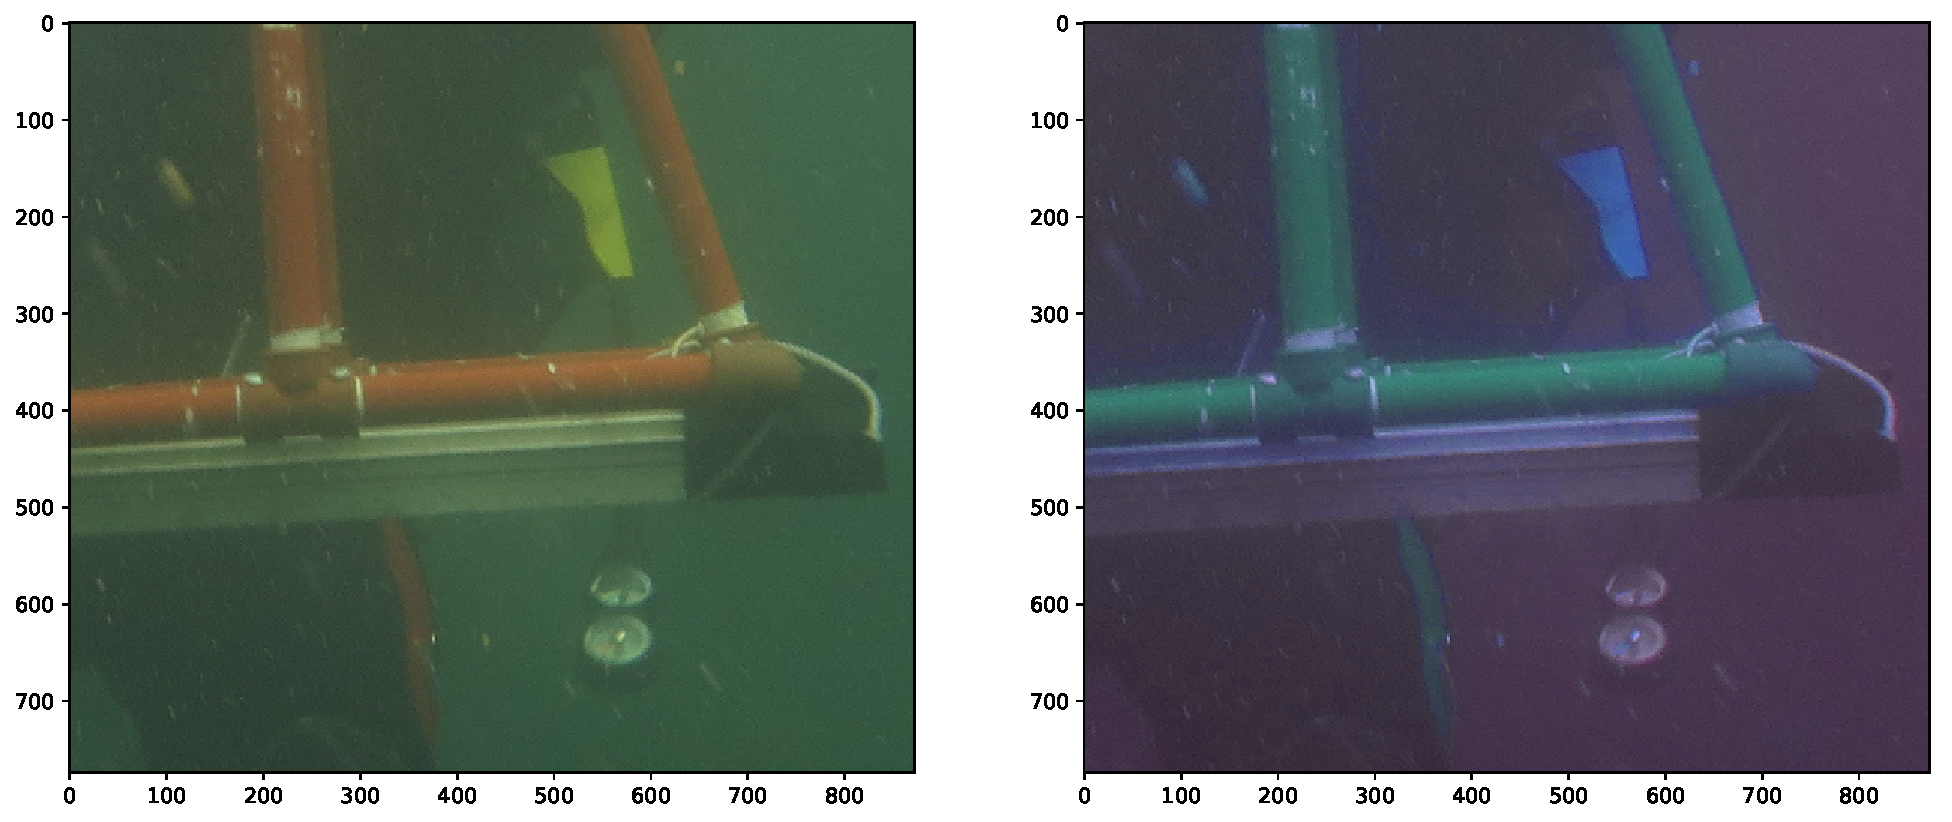
\includegraphics[height=6cm]{informe-imgs/ej03-2.pdf}
  \caption{\texttt{python3 practica1/ej03-a.py 2.5 test/imagenesClaseColor/1907xx.png --end}}
\end{figure}

$c = 4.5$
\begin{figure}[H]
\centering
  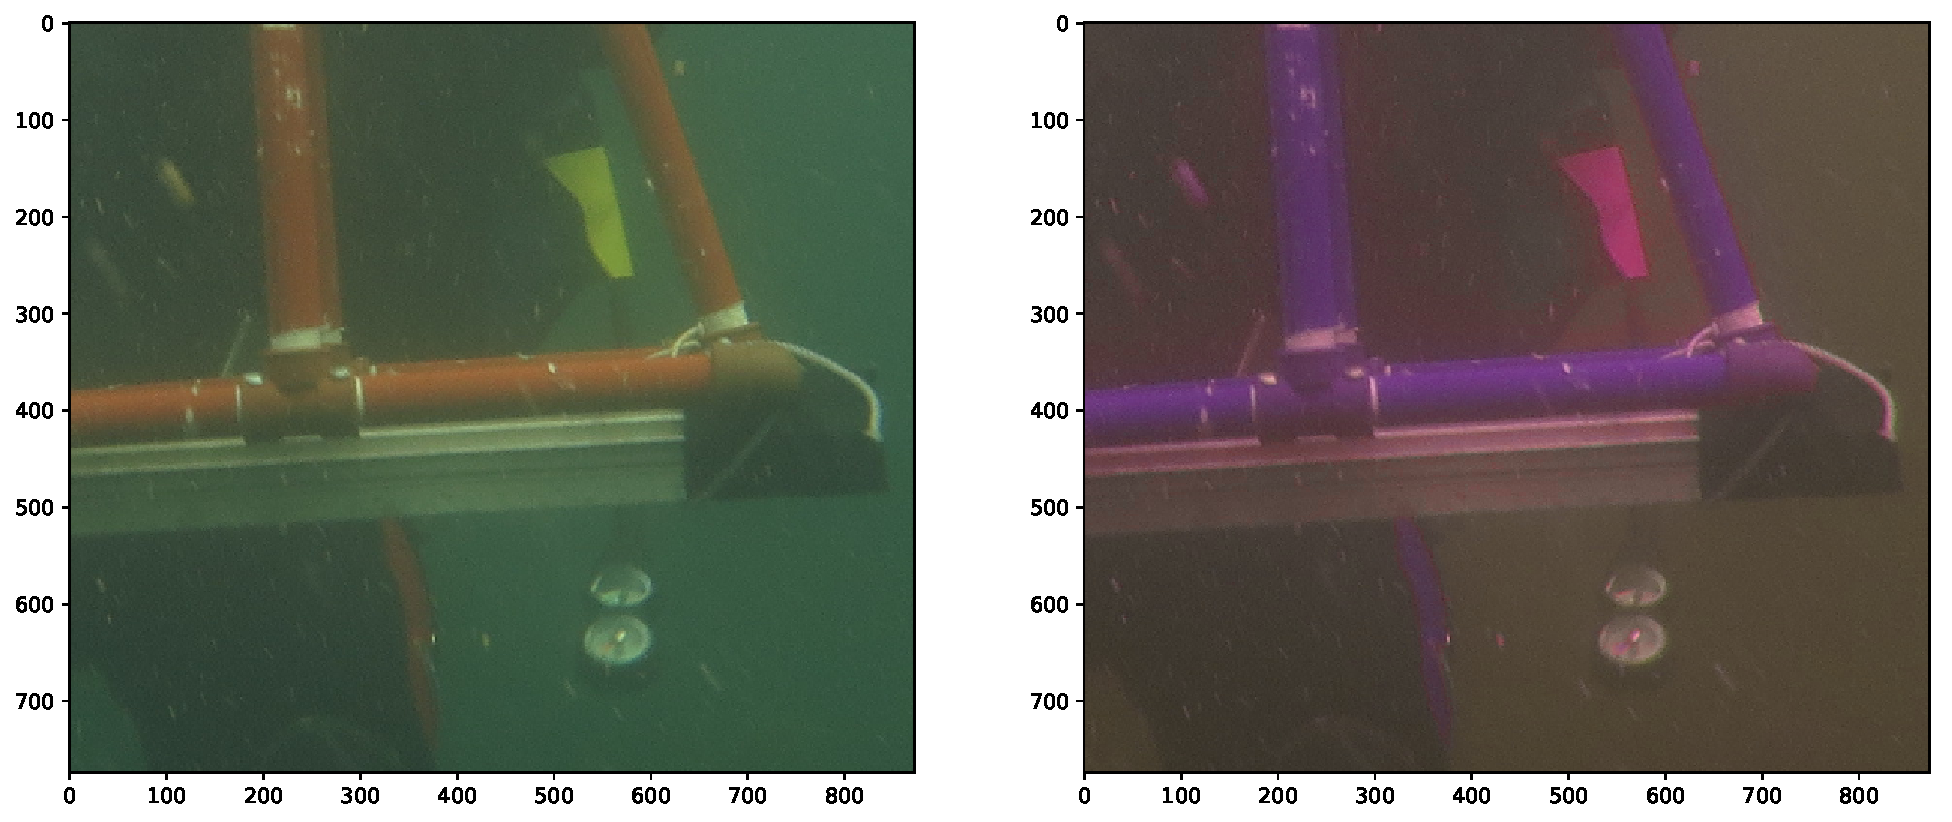
\includegraphics[height=6cm]{informe-imgs/ej03-3.pdf}
  \caption{\texttt{python3 practica1/ej03-a.py 4.5 test/imagenesClaseColor/1907xx.png --end}}
\end{figure}

\subsubsection*{Imagen 2 -- 1901xx}
$c = 0.5$
\begin{figure}[H]
\centering
  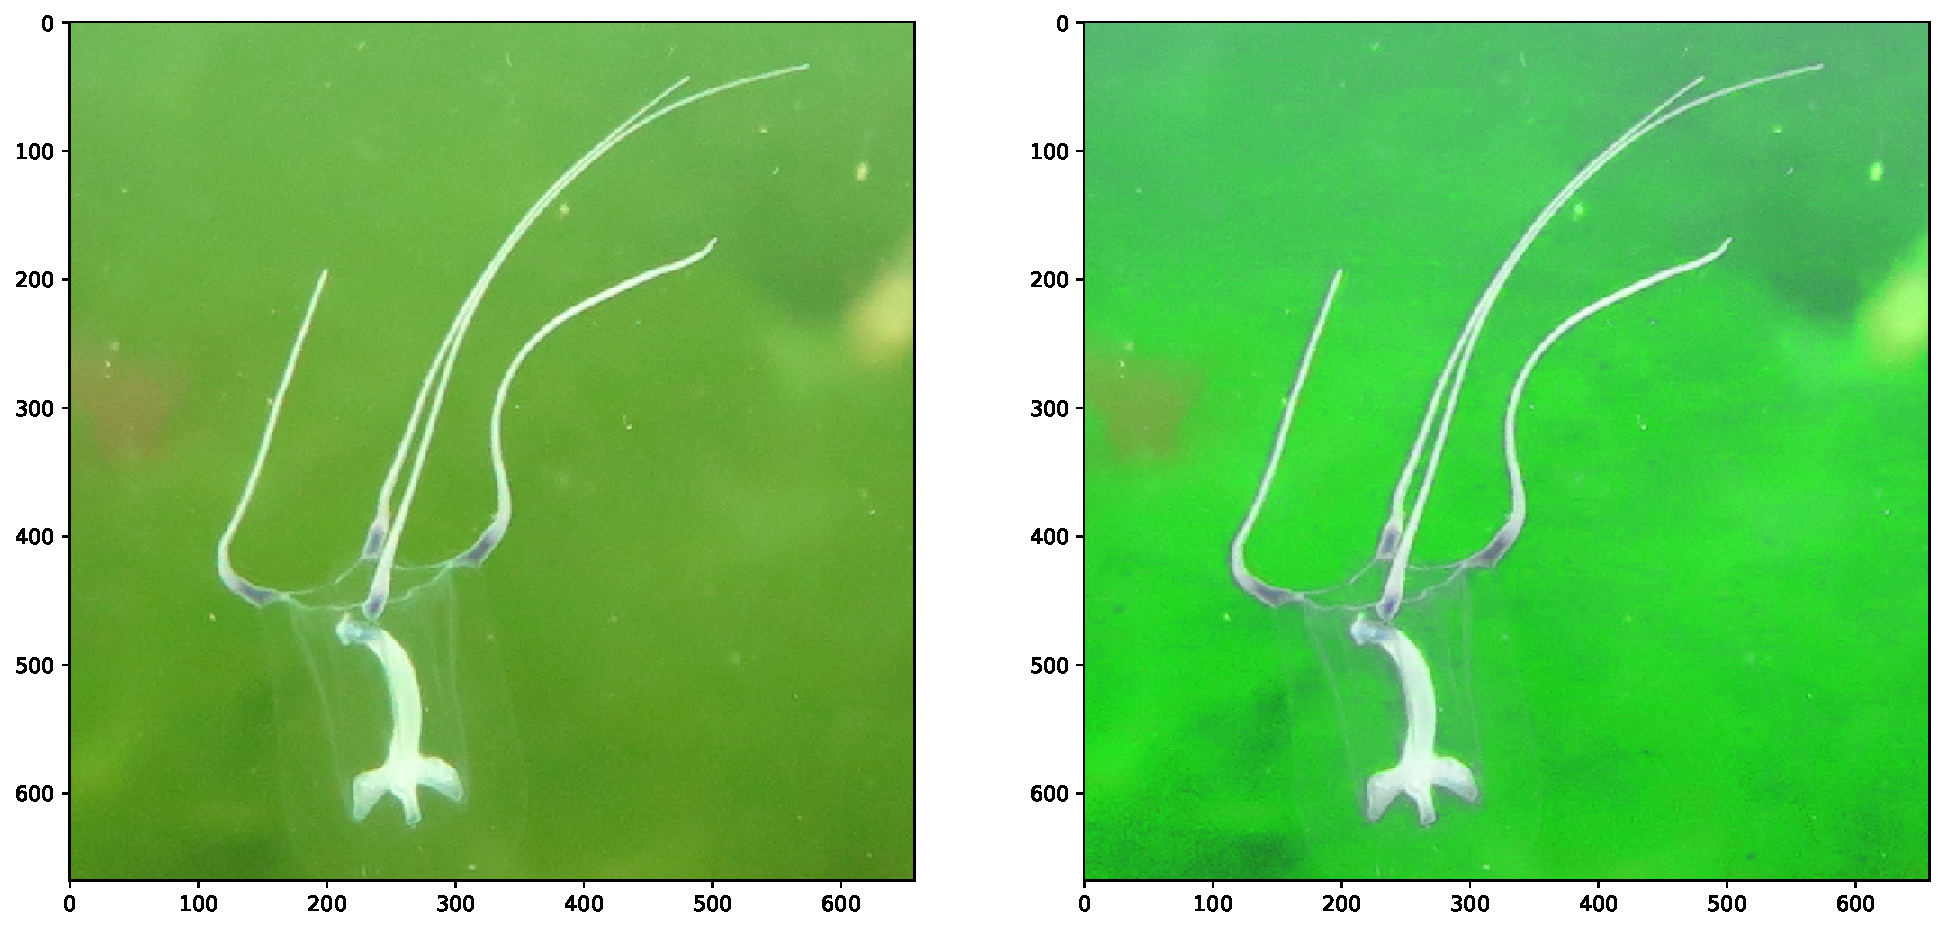
\includegraphics[height=6cm]{informe-imgs/ej03-4.pdf}
  \caption{\texttt{python3 practica1/ej03-a.py 0.5 test/imagenesClaseColor/1901xx.png --end}}
\end{figure}

$c = 2.5$
\begin{figure}[H]
\centering
  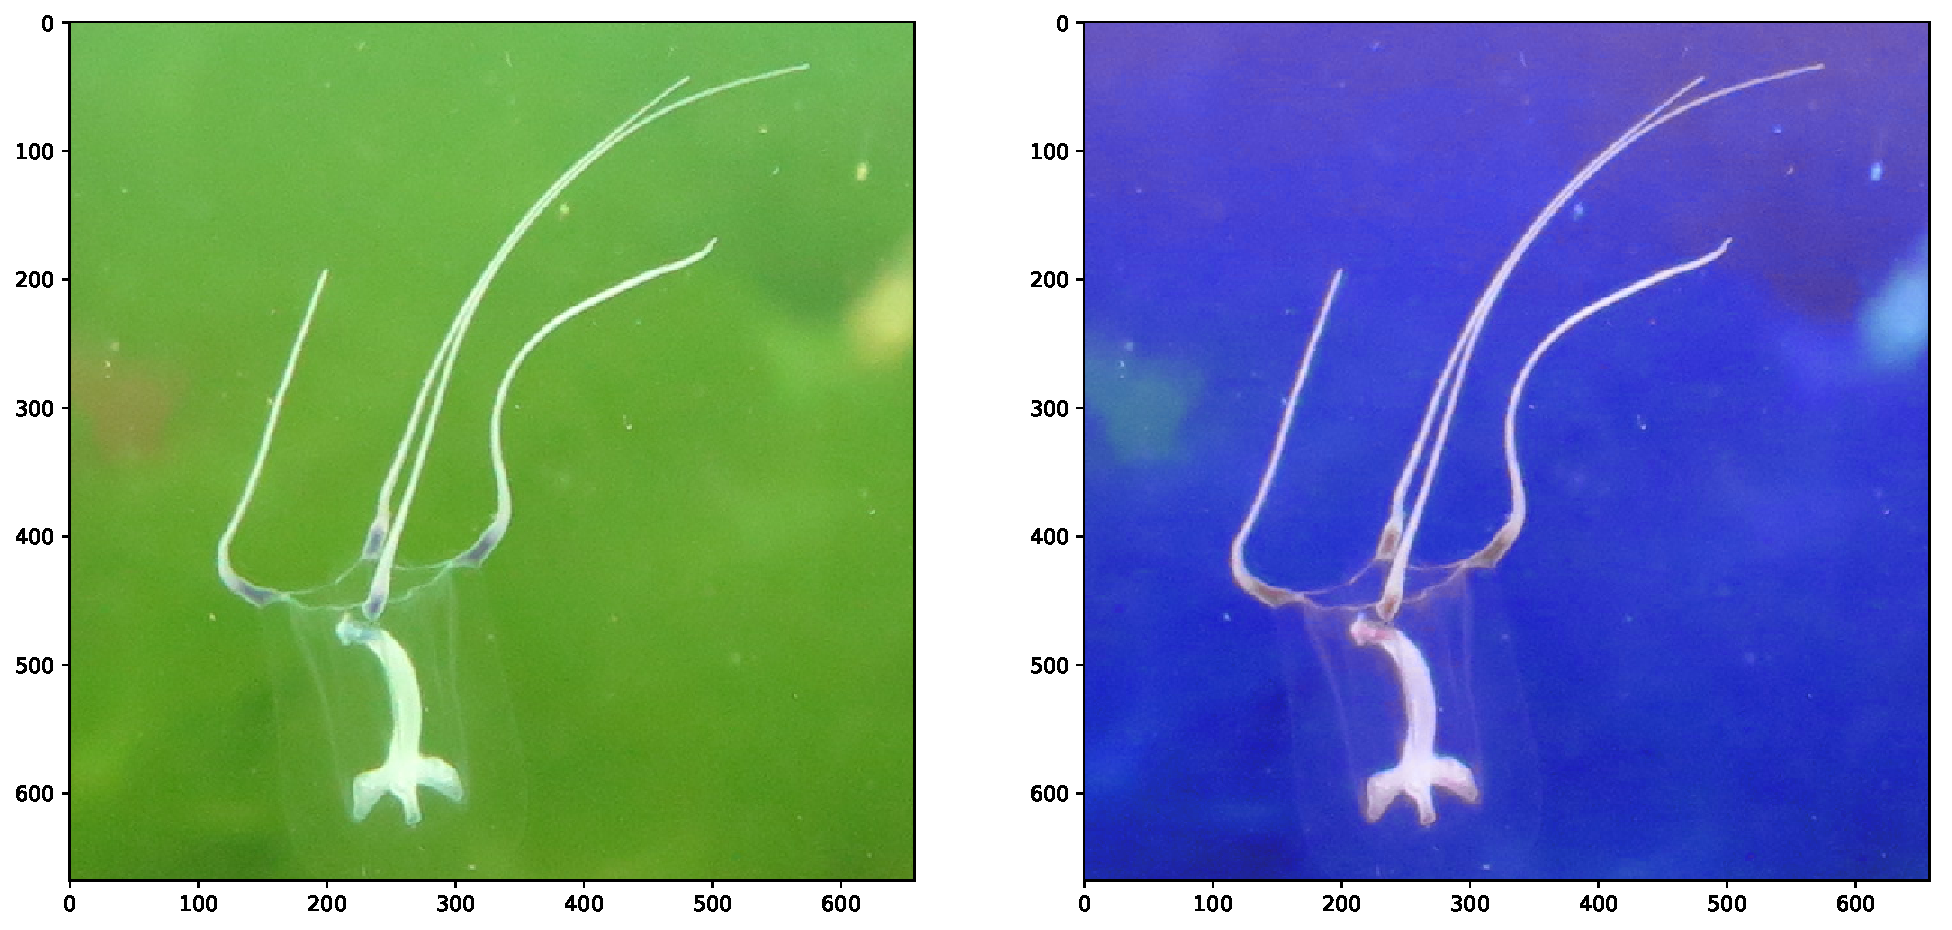
\includegraphics[height=6cm]{informe-imgs/ej03-5.pdf}
  \caption{\texttt{python3 practica1/ej03-a.py 2.5 test/imagenesClaseColor/1901xx.png --end}}
\end{figure}

$c = 4.5$
\begin{figure}[H]
\centering
  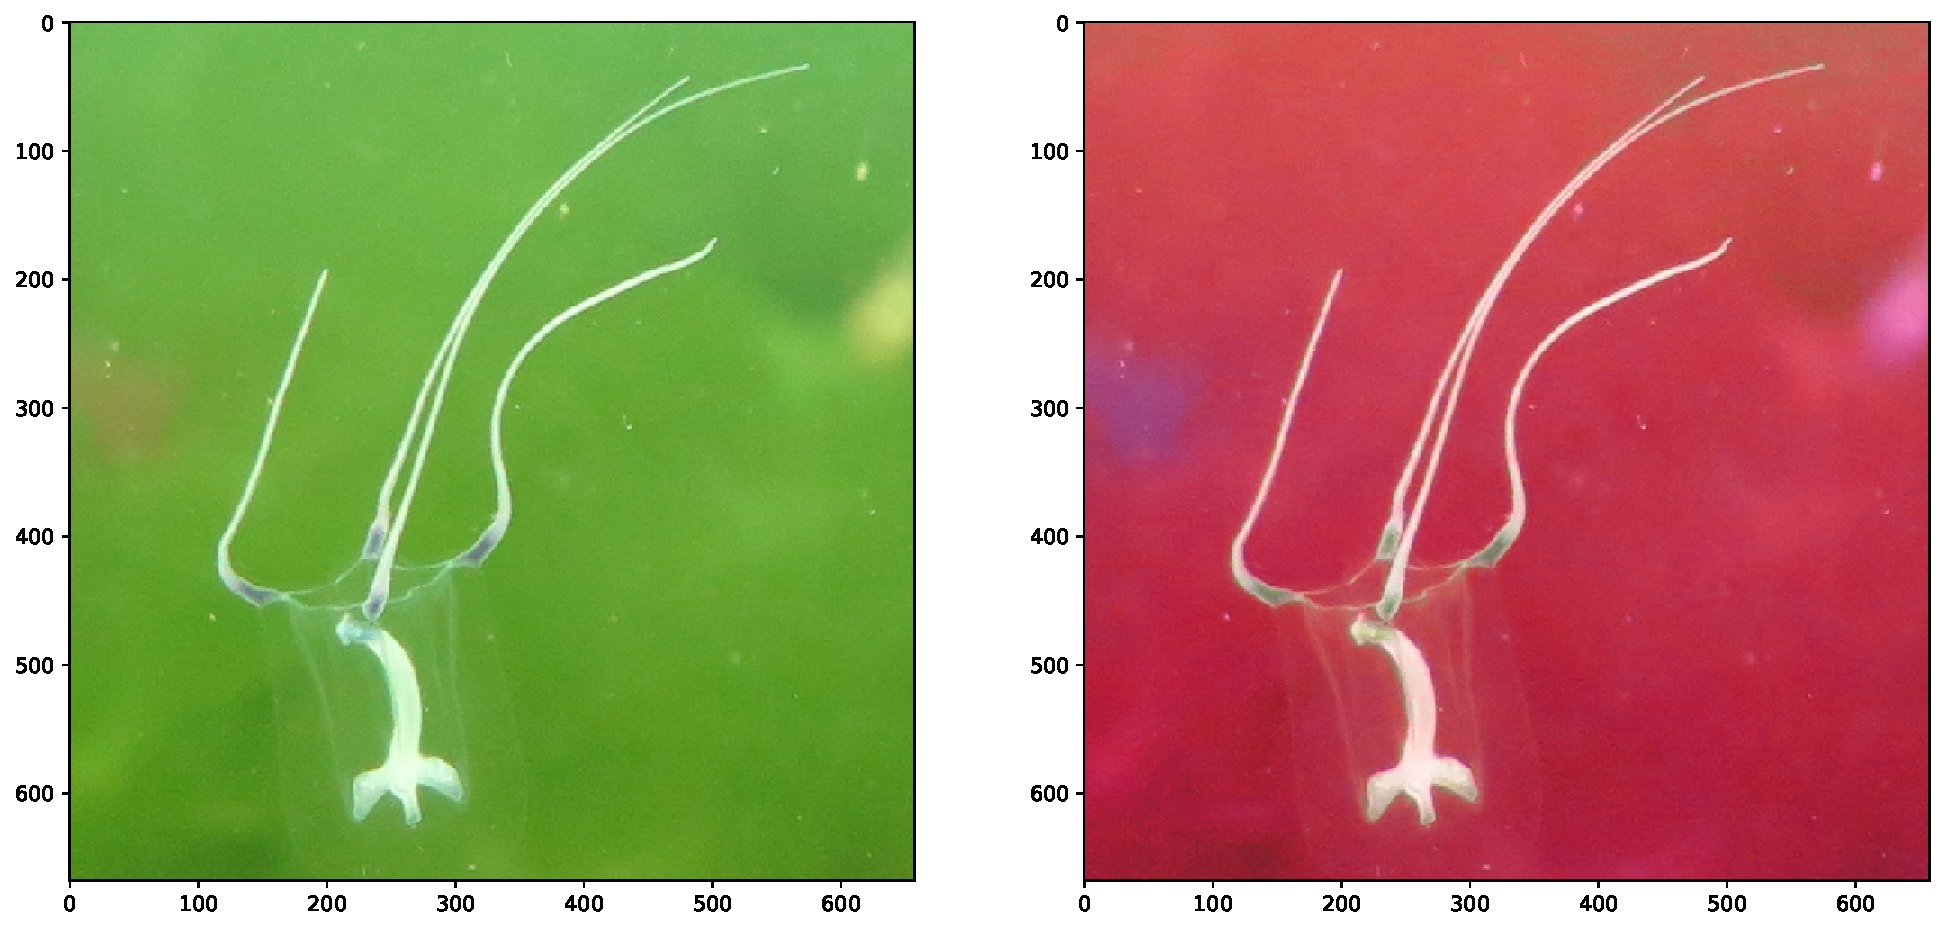
\includegraphics[height=6cm]{informe-imgs/ej03-6.pdf}
  \caption{\texttt{python3 practica1/ej03-a.py 4.5 test/imagenesClaseColor/1901xx.png --end}}
\end{figure}

\newpage

\section{Ejercicio 4.}

\subsection{Ejercicio 4.a. Dónde son mas visibles los detalles y el ruido.}
\begin{figure}[H]
\centering
  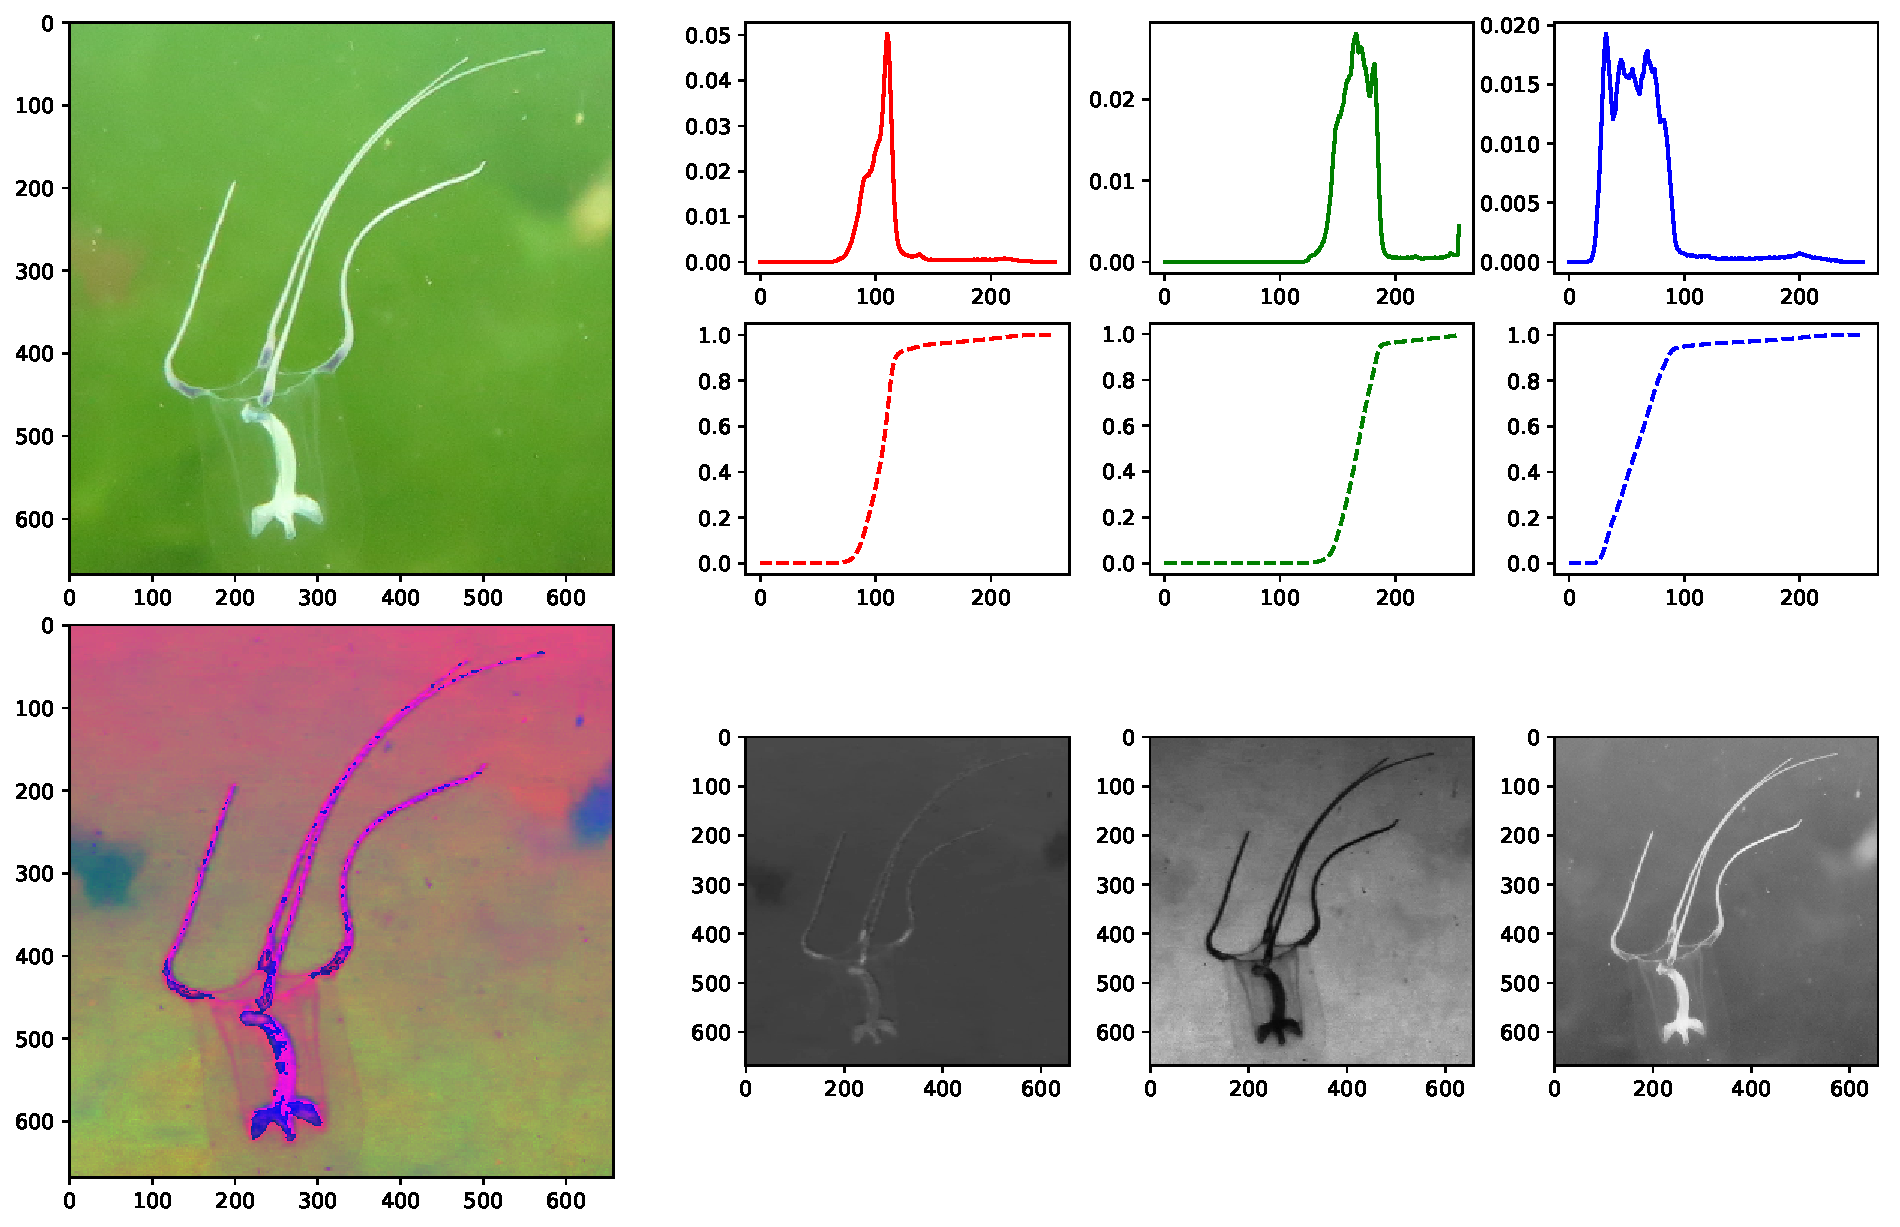
\includegraphics[height=8cm]{informe-imgs/ej04-1.pdf}
  \caption{\texttt{python3 practica1/ej01-c.py test/imagenesClaseColor/1901xx.png}}
\end{figure}
\begin{figure}[H]
\centering
  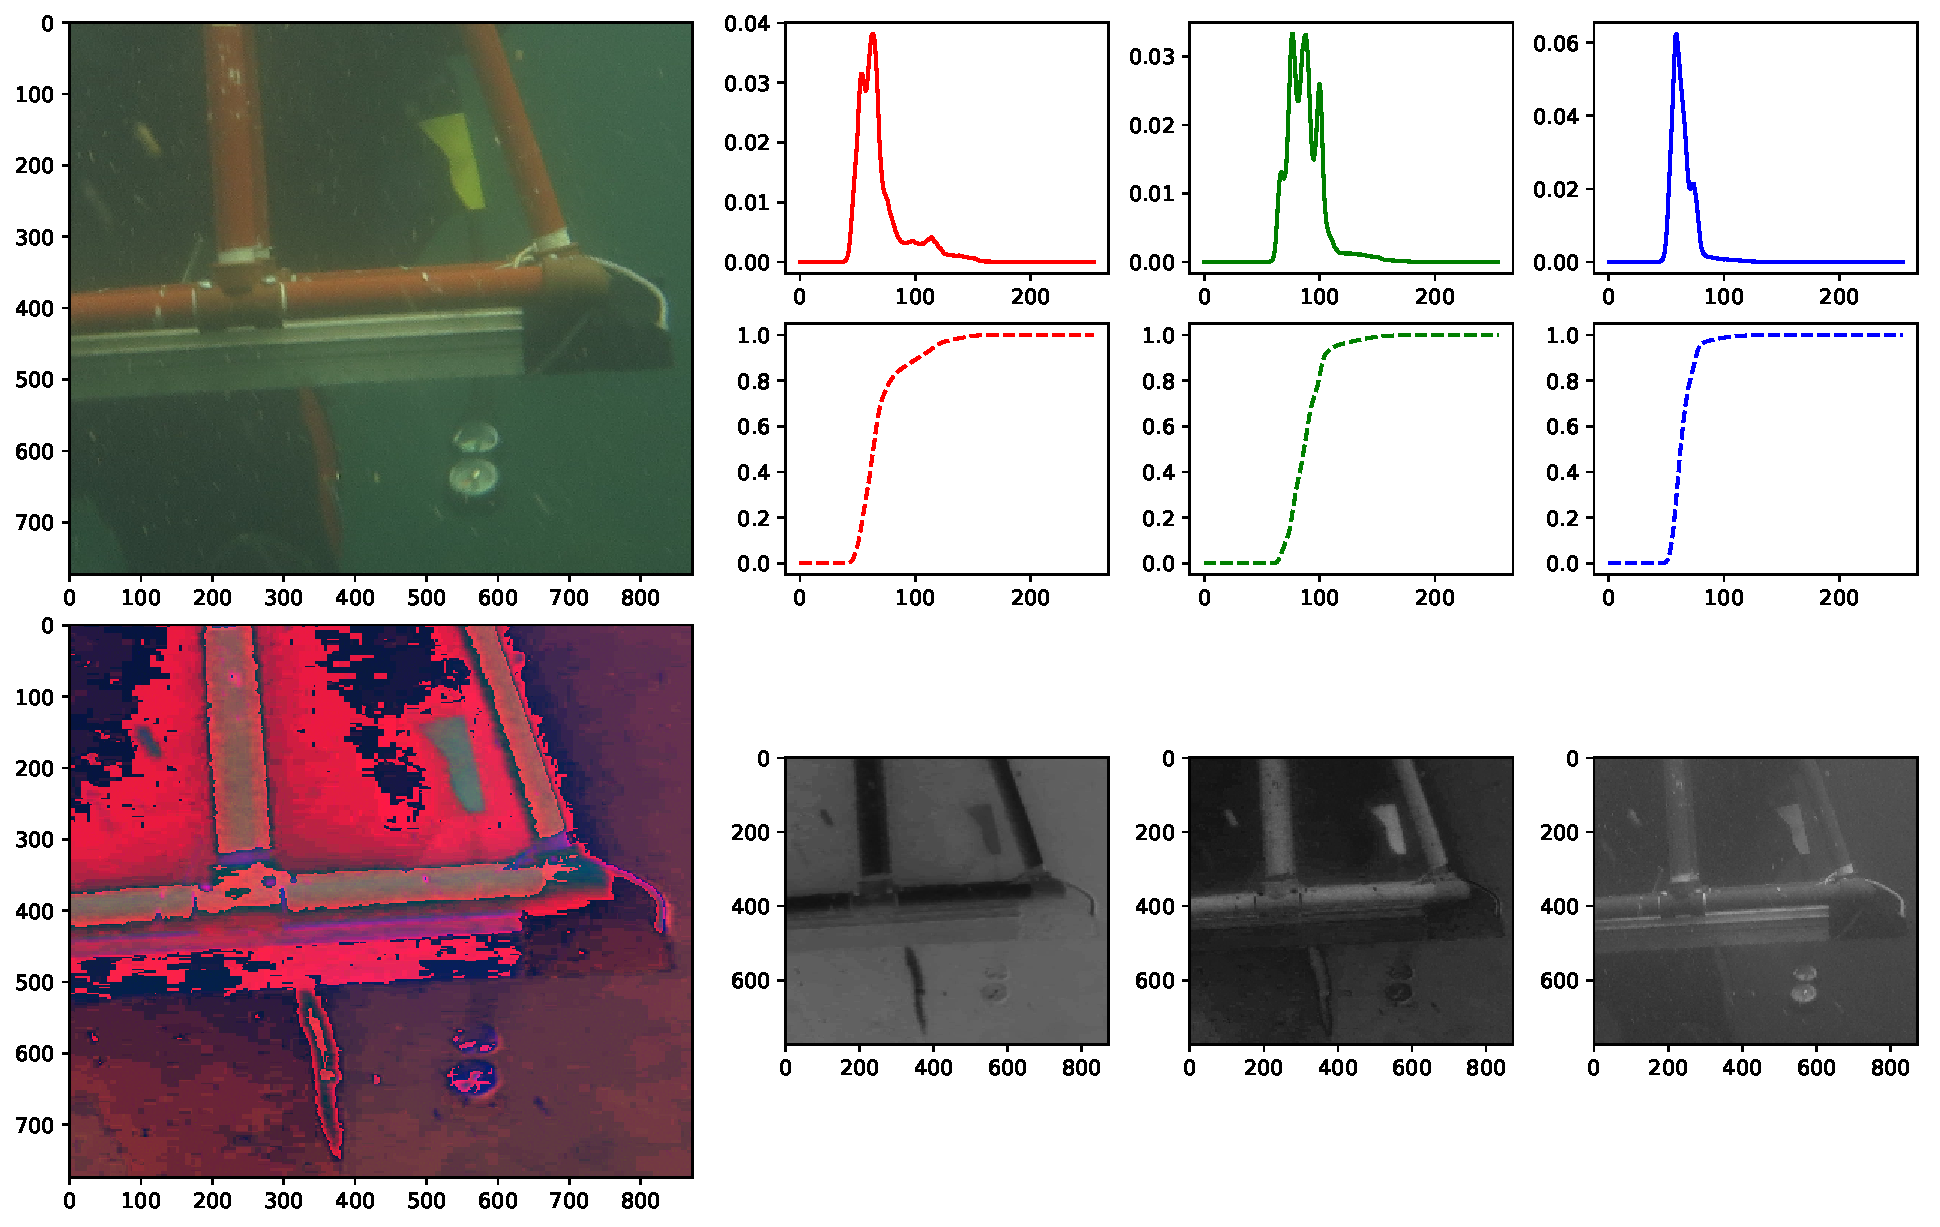
\includegraphics[height=8cm]{informe-imgs/ej04-2.pdf}
  \caption{\texttt{python3 practica1/ej01-c.py test/imagenesClaseColor/1901xx.png}}
\end{figure}
\begin{figure}[H]
\centering
  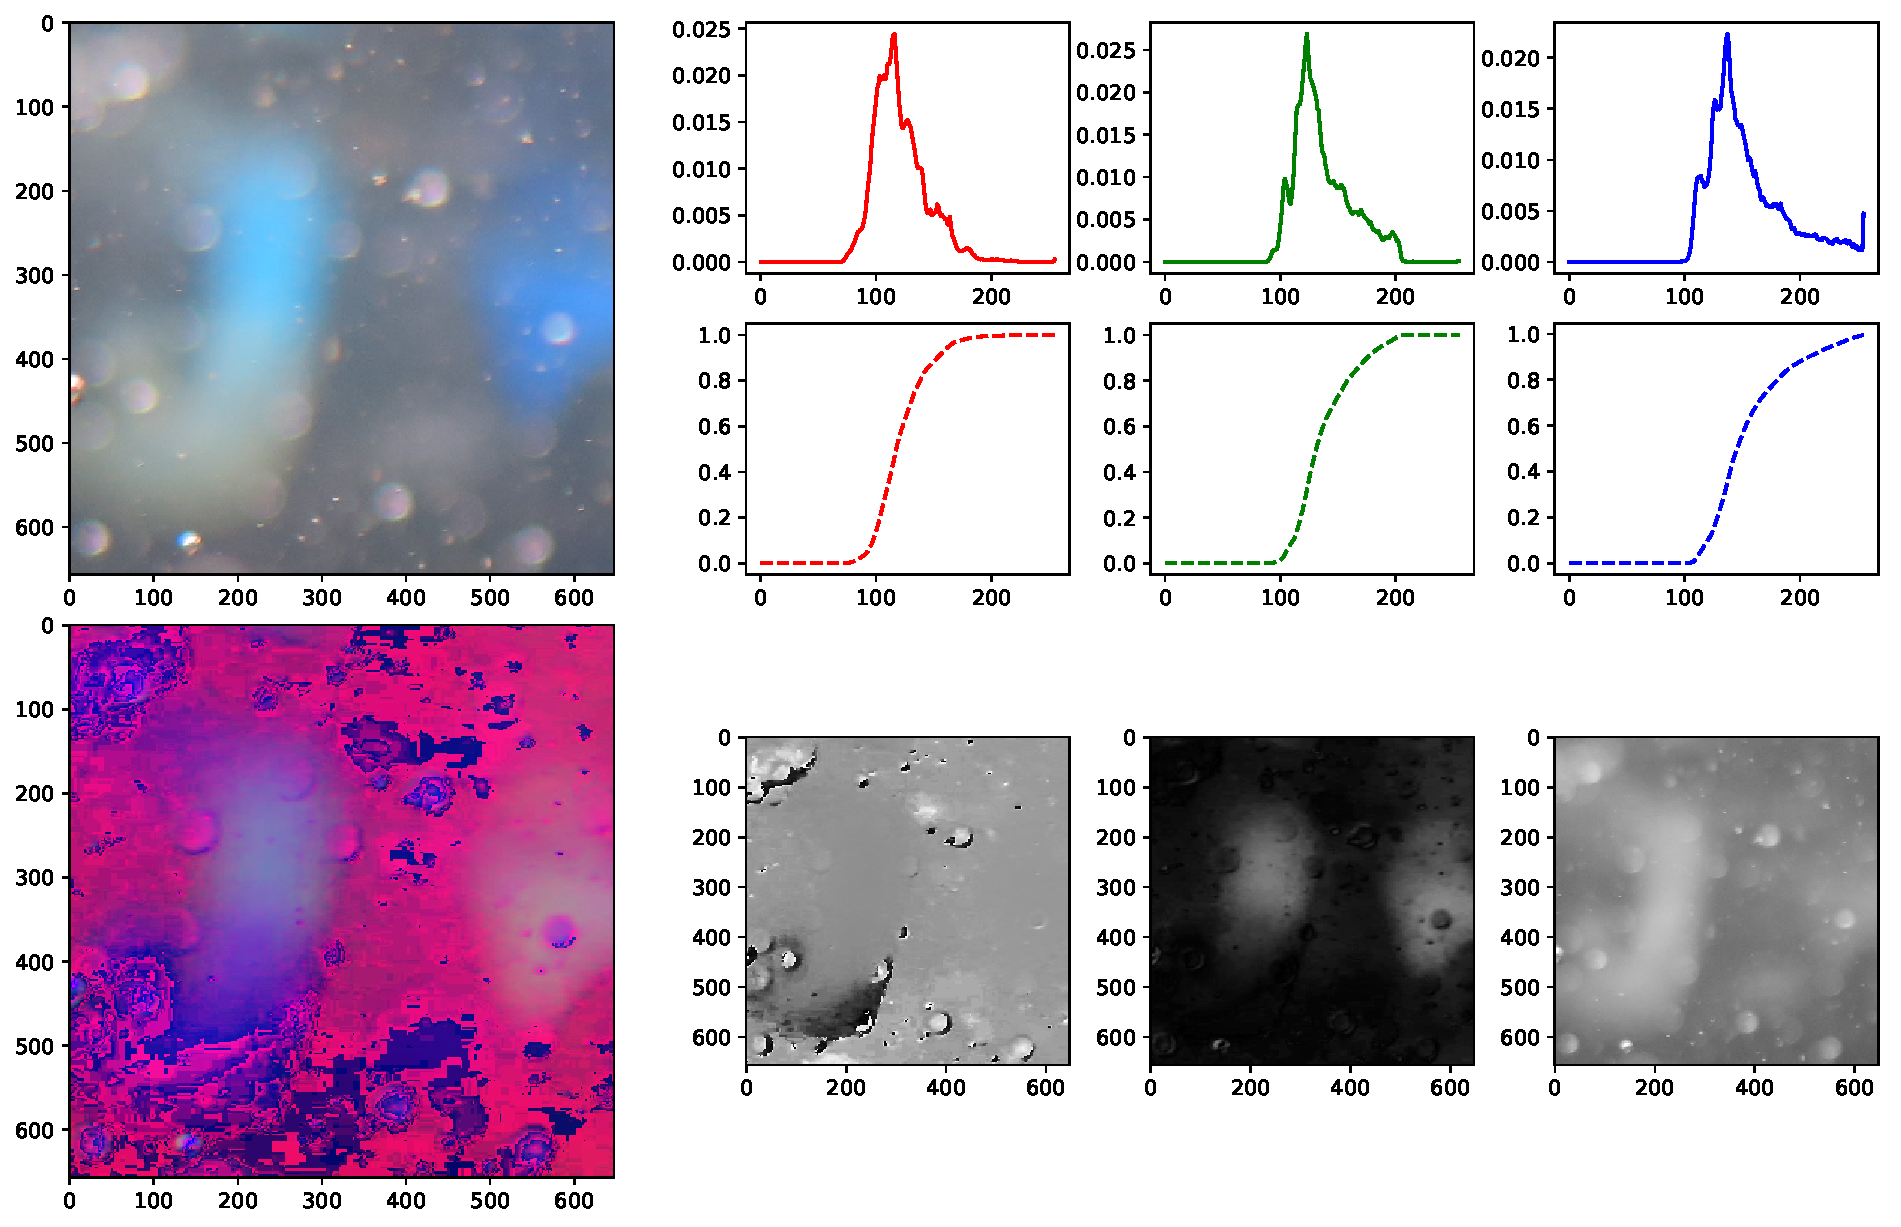
\includegraphics[height=8cm]{informe-imgs/ej04-3.pdf}
  \caption{\texttt{python3 practica1/ej01-c.py test/imagenesClaseColor/1923xx.png}}
\end{figure}

Como puede observarse, los detalles se notan más en el canal I, o sea, en la intensidad.
Por otro lado, el ruido se observa más en el canal S, de saturación: a más ruido menos saturación.

\subsection{Ejercicio 4.b. Dónde afectan más los bordes difuminados.}
\begin{figure}[H]
\centering
  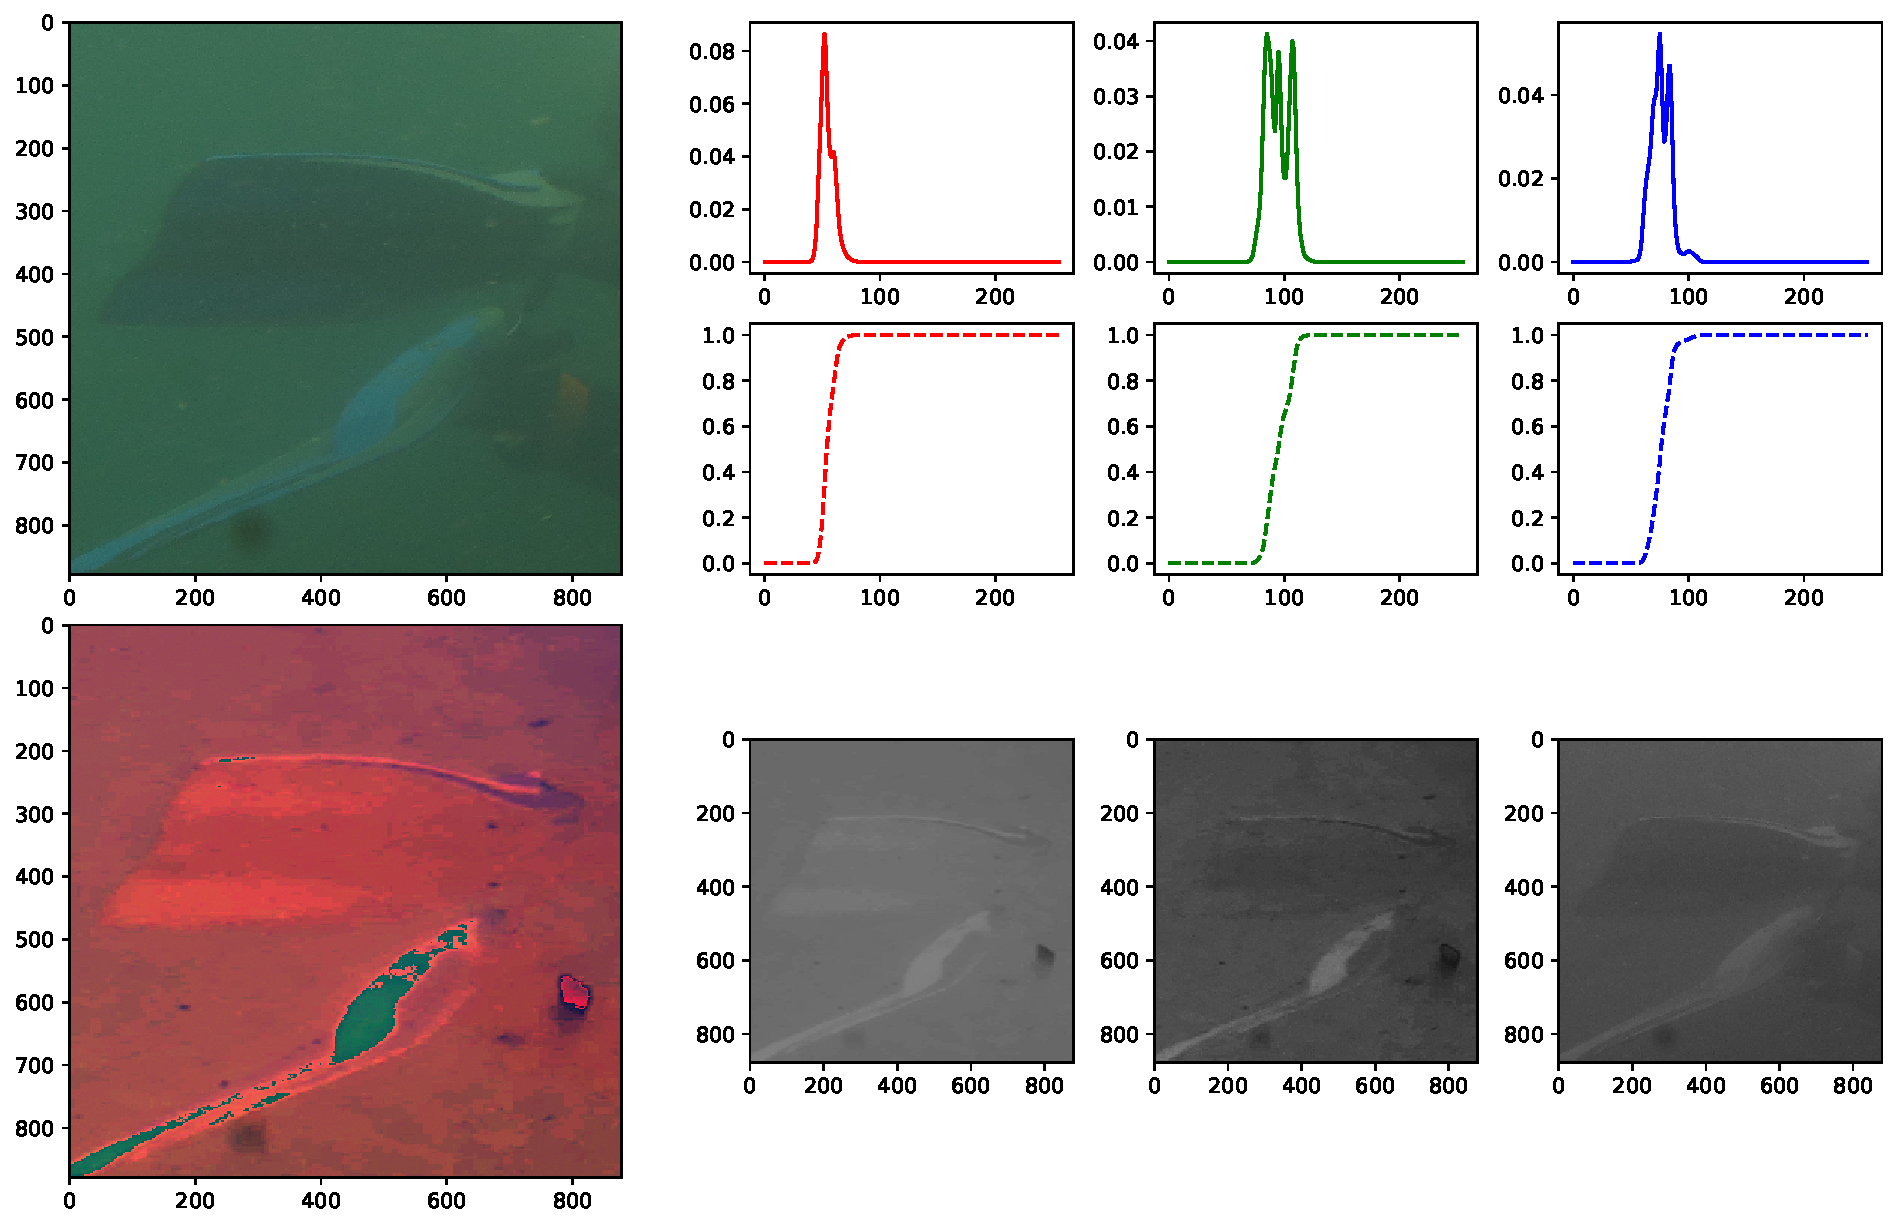
\includegraphics[height=8cm]{informe-imgs/ej04-4.pdf}
  \caption{\texttt{python3 practica1/ej01-c.py test/imagenesClaseColor/1908xxx.png}}
\end{figure}
\begin{figure}[H]
\centering
  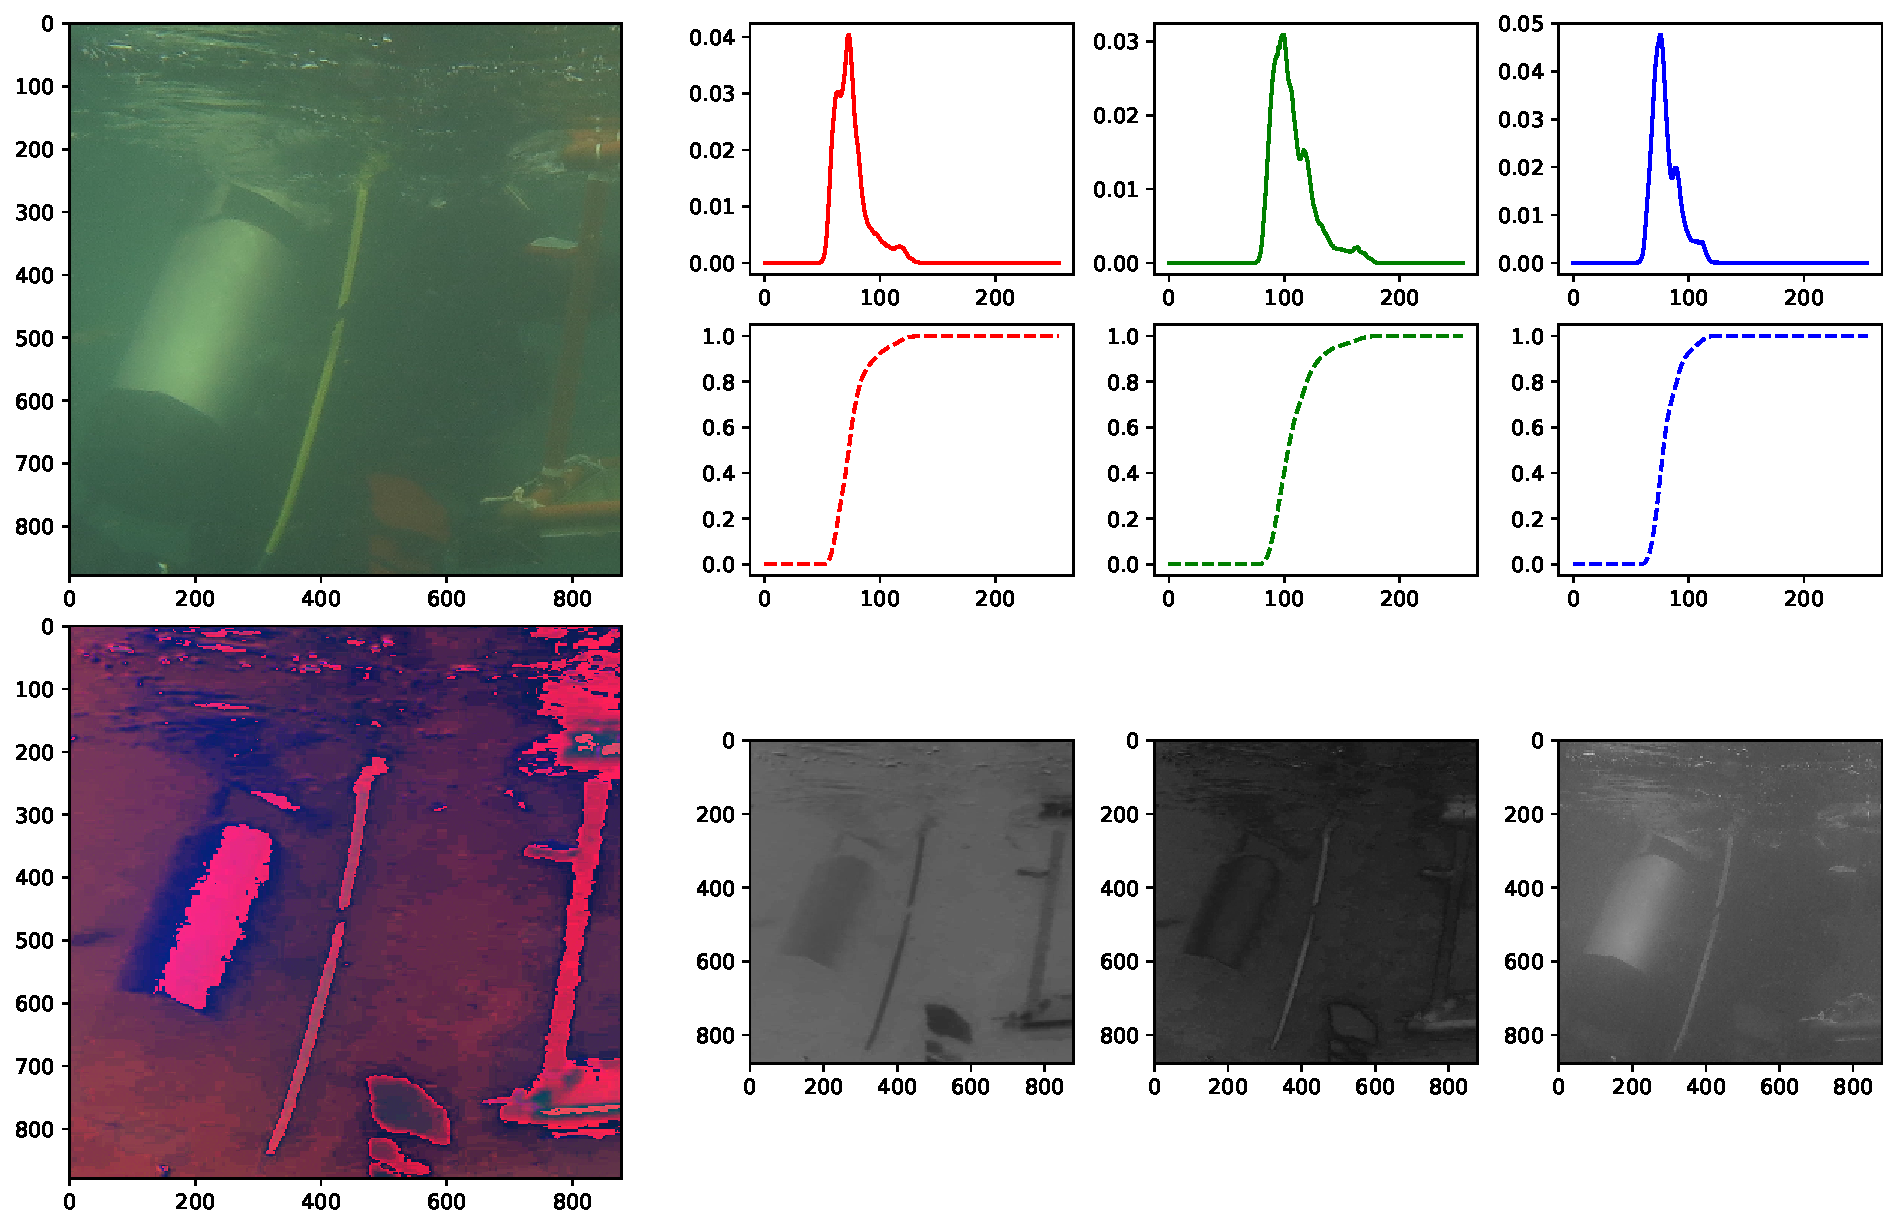
\includegraphics[height=8cm]{informe-imgs/ej04-5.pdf}
  \caption{\texttt{python3 practica1/ej01-c.py test/imagenesClaseColor/1908xx.png}}
\end{figure}

Los bordes difuminados se notan más en el canal S, de saturación, pues los bordes difuminados tienen baja saturación (no
hay colores puros).

\end{document}

